% =============================================================================
%  Dos barreras para el acceso equitativo — version ES
%  Version espaniola, equivalente en contenido a privacidad_UAIS_en.tex.
%  Comparte el mismo .bib y las mismas figuras (texto interno en ingles).
% =============================================================================
\documentclass[pdflatex,sn-basic,Numbered]{sn-jnl}

\usepackage{graphicx}
\usepackage{multirow}
\usepackage{amsmath,amssymb,amsfonts}
\usepackage{amsthm}
\usepackage{mathrsfs}
\usepackage[title]{appendix}
\usepackage{xcolor}
\usepackage{textcomp}
\usepackage{manyfoot}
\usepackage{booktabs}
\usepackage{longtable}
\usepackage{array}
\usepackage{ragged2e}
\usepackage{pifont}
\usepackage{float}
\usepackage[spanish,es-tabla,es-noshorthands]{babel}

\definecolor{gris}{gray}{0.35}
\newcommand{\si}{\ding{51}}
\newcommand{\no}{\textcolor{gris}{\textbf{--}}}
\newcommand{\pc}{\textbf{P}}
\newcommand{\nv}{\textsl{\footnotesize NV}}

\theoremstyle{thmstyleone}
\newtheorem{theorem}{Teorema}
\newtheorem{proposition}[theorem]{Proposici\'on}
\theoremstyle{thmstyletwo}
\newtheorem{example}{Ejemplo}
\newtheorem{remark}{Observaci\'on}
\theoremstyle{thmstylethree}
\newtheorem{definition}{Definici\'on}

\raggedbottom

\begin{document}

\title[Dos barreras para el acceso equitativo]{Dos barreras para el acceso equitativo: conformidad {WCAG} y rastreo previo al consentimiento en los sitios web de universidades ecuatorianas y de \'elite internacional}

\author*[1]{\fnm{Gleiston} \sur{Guerrero-Ulloa}}\email{gguerrero@uteq.edu.ec}
\author[2]{\fnm{Andrea} \sur{Z\'u\~niga Paredes}}\email{andrear.zuniga@educacion.gob.ec}
\author[1]{\fnm{Efra\'in} \sur{D\'iaz-Mac\'ias}}\email{efraindiaz@uteq.edu.ec}

\affil*[1]{\orgdiv{Facultad de Ciencias de la Computaci\'on}, \orgname{Universidad T\'ecnica Estatal de Quevedo}, \orgaddress{\street{Av.\ Quito Km 1.5 v\'ia a Santo Domingo de los Ts\'achilas}, \city{Quevedo}, \postcode{120302}, \state{Los R\'ios}, \country{Ecuador}}}
\affil[2]{\orgname{Ministerio de Educaci\'on del Ecuador}, \orgaddress{\city{Quito}, \postcode{170518}, \state{Pichincha}, \country{Ecuador}}}

\abstract{\textbf{Prop\'osito.} Quien quiere estudiar postula y se matricula por el sitio web de la universidad, y un obst\'aculo puesto ah\'i lo deja fuera. Estudiamos dos de esos obst\'aculos, si una persona con discapacidad puede usar el sitio y c\'omo trata los datos personales, y preguntamos qui\'en decide la protecci\'on de cada visitante.\\[4pt]
\textbf{M\'etodos.} Examinamos las portadas de 126 universidades: las 63 reconocidas en el Ecuador y 63 de las mejor situadas del mundo. En cada una leimos el aviso de privacidad e hicimos una comprobaci\'on autom\'atica en navegador real, contando los incumplimientos de las Pautas de Accesibilidad para el Contenido Web (WCAG) y cada cookie depositada antes de que la persona aceptara nada. La repetimos desde el Ecuador, Alemania, el Reino Unido y los Estados Unidos.\\[4pt]
\textbf{Resultados.} Las universidades ecuatorianas publican menos: el 61,9\,\% ten\'ia aviso de privacidad y el 38,1\,\% un contacto para asuntos de privacidad, frente al 93,7\,\% y el 85,7\,\% de las mejor situadas. Ambos grupos fallaron en accesibilidad; los ecuatorianos m\'as en el nivel b\'asico, el 45\,\% frente al 19\,\%. El rastreo previo al consentimiento fue parecido en ambos grupos, pero cambi\'o con el pa\'is del visitante: el 67,8\,\% de los sitios rastre\'o a quien estaba en el Ecuador y el 60,3\,\% a quien estaba en Alemania. Esa diferencia la marcaron las empresas que proveen el c\'odigo de rastreo, no las universidades: Microsoft, TapAd y StackAdapt no pusieron cookie alguna a los visitantes europeos y brit\'anicos mientras rastreaban a los ecuatorianos y estadounidenses.\\[4pt]
\textbf{Conclusi\'on.} Las debilidades del Ecuador est\'an en lo que publican las universidades y en la accesibilidad b\'asica. Pero cu\'anto rastreo encuentra una persona no lo decide la universidad ni la ley que la obliga, sino unas listas de pa\'ises que mantienen las empresas de publicidad: la misma p\'agina protege a unos y a otros no, solo seg\'un d\'onde est\'en.}

\keywords{accesibilidad web, conformidad WCAG, protecci\'on de datos personales, consentimiento de cookies, sitios web universitarios, Ecuador}

\maketitle

% =============================================================================
\section{Introducci\'on}\label{sec:introduction}
% =============================================================================

El sitio web institucional es el canal por el que una persona interesada encuentra la informaci\'on de las carreras, presenta su postulaci\'on, completa la matr\'icula y llega a los servicios de biblioteca, tutor\'ia y administraci\'on. Una barrera incrustada en ese canal no es, por tanto, un defecto cosm\'etico, sino una restricci\'on del acceso a la instituci\'on. La investigaci\'on sobre acceso universal lleva tiempo planteando esto como un problema de dise\~no y no de remediaci\'on: los entornos y los servicios deber\'ian ser utilizables por el mayor rango posible de personas desde el origen, y las normas de accesibilidad son la expresi\'on operativa de ese principio para los productos digitales \citep{hermosaramirez2025universal}. Las Pautas de Accesibilidad para el Contenido Web (WCAG), en su versi\'on 2.2 vigente \citep{wcag22}, aportan los criterios verificables, y varios reg\'imenes legales las hacen obligatorias, entre ellos la \emph{European Accessibility Act} \citep{eaa2019} y, en los Estados Unidos, la \emph{Americans with Disabilities Act} y la Secci\'on 508 de la \emph{Rehabilitation Act} \citep{ada1990,section508}.

La protecci\'on de datos personales es una segunda barrera que opera sobre el mismo canal y, sostenemos, sobre el mismo principio. Quien debe aceptar un rastreo no explicado para consultar una oferta acad\'emica, o no logra averiguar qui\'en trata los datos de su postulaci\'on ni c\'omo oponerse, afronta un costo de participaci\'on que se reparte de forma desigual: recae con m\'as fuerza sobre quienes tienen menor alfabetizaci\'on jur\'idica, menos medios t\'ecnicos para negarse y menos posibilidad de acudir a otro proveedor. Le\'idas as\'i, la gobernanza opaca de la privacidad y las interfaces inaccesibles son dos mecanismos de un mismo fen\'omeno, a saber, el costo desigual de usar un servicio de cara al p\'ublico. Ese encuadre justifica estudiarlas juntas y no como dos listas de verificaci\'on separadas.

El trabajo emp\'irico ha tratado ambas literaturas por separado. En accesibilidad, las auditor\'ias de portales universitarios documentan barreras generalizadas en las universidades mejor posicionadas evaluadas con WCAG 2.2 \citep{krittika2025accessibility}, en las europeas \citep{krejtz2025higher}, en la regi\'on del Golfo \citep{fakrudeen2025evaluation} y en los servicios p\'ublicos en l\'inea en general \citep{aljedaani2025egovernment,iniesto2025service}, con un rezago latinoamericano documentado desde hace a\~nos \citep{campoverdemolina2023accessibility,acostavargas2020dataset}. En privacidad, la medici\'on a gran escala ha establecido que la norma escrita y el comportamiento observado avanzan a ritmos distintos: el Reglamento General de Protecci\'on de Datos (RGPD) \citep{gdpr2016} multiplic\'o avisos y banners sin un cambio proporcional en el rastreo \citep{degeling2019value,trevisan2019four,kretschmer2021cookie}, las interfaces de consentimiento incumplen a menudo las condiciones legales de un consentimiento v\'alido \citep{matte2020cookie,nouwens2020dark,gray2021dark,habib2022okay}, los gestores de cookies con frecuencia no bloquean lo que dicen bloquear \citep{sanchezrola2019can,bollinger2022automating} y, en la educaci\'on superior en concreto, se ha observado que las pol\'iticas cambian para parecer conformes antes que para serlo \citep{munot2025compliance}. Hasta donde alcanza nuestro conocimiento, ning\'un estudio ha medido ambas barreras sobre el mismo conjunto de sitios institucionales, con el mismo protocolo y en la misma fecha.

El Ecuador es un escenario informativo para esa medici\'on. Su Ley Org\'anica de Protecci\'on de Datos Personales (LOPDP) entr\'o en vigor en 2021 y solo se reglament\'o en 2023 \citep{lopdp2021,reglamentolopdp2023}, lo que la sit\'ua en la oleada m\'as reciente de un proceso de difusi\'on regional que la literatura comparada ha mostrado desigual en compromiso y en aplicaci\'on \citep{carrillo2022follow,chavarriamora2025lack}. El pa\'is tiene, adem\'as, una poblaci\'on cerrada y enumerable de 63 IES reconocidas, lo que permite un censo completo en lugar de una muestra.

Este art\'iculo aborda cuatro preguntas de investigaci\'on.

\begin{itemize}
	\item \textbf{PI1.} ¿En qu\'e se diferencian las IES ecuatorianas y un grupo internacional de referencia en la gobernanza de la privacidad visible en su portada, esto es, un aviso publicado, un marco legal citado, una enumeraci\'on de derechos y un canal de contacto identificado?
	\item \textbf{PI2.} ¿En qu\'e se diferencian ambos grupos en el comportamiento previo al consentimiento, es decir, en las cookies depositadas antes de toda interacci\'on con una interfaz de consentimiento, observados los dos desde el mismo punto fuera de la Uni\'on Europea?
	\item \textbf{PI3.} ¿En qu\'e se diferencian ambos grupos en la conformidad WCAG detectable de forma autom\'atica, y la diferencia est\'a en el volumen de fallos o en el nivel de conformidad en que ocurren?
	\item \textbf{PI4.} Dentro de cada grupo, ¿la accesibilidad medida se asocia con una mayor contenci\'on en el rastreo previo al consentimiento?
	\item \textbf{PI5.} ¿El comportamiento previo al consentimiento de una misma p\'agina depende de d\'onde se encuentre el \emph{visitante} y, de ser as\'i, la frontera sigue a la ley que obliga a la instituci\'on o a otra cosa?
\end{itemize}

Las contribuciones son las siguientes. Primera, una medici\'on pareada de accesibilidad y rastreo previo al consentimiento sobre 126 portadas universitarias con un protocolo \'unico, plenamente especificado y reproducible, publicado junto con su configuraci\'on, su taxonom\'ia de cookies de rastreo y su salida cruda. Segunda, un reanalisis inferencial que separa las diferencias que el dise\~no puede sostener de las que no, con una prueba de equivalencia expl\'icita y una declaraci\'on de potencia para los resultados nulos que el estudio informa. Tercera, una replicaci\'on de la auditor\'ia en vivo desde cuatro puntos de observaci\'on, el Ecuador, Alemania, el Reino Unido y los Estados Unidos, que convierte una conjetura jur\'idica en una medici\'on: se muestra que la protecci\'on que recibe una persona depende de d\'onde est\'a ella y que la aplican los proveedores publicitarios, no las instituciones ni la ley que las obliga. Cuarta, un mapeo indicador por jurisdicci\'on que separa la conducta observada del incumplimiento legal, dado que la mayor\'ia de las once jurisdicciones estudiadas no impone un deber general de consentimiento previo para las cookies.

El resto del art\'iculo se organiza como sigue. La Secci\'on~\ref{sec:related} revisa ambas literaturas y enuncia la brecha. La Secci\'on~\ref{sec:methods} describe el dise\~no, el muestreo, el libro de c\'odigos, el protocolo de auditor\'ia y el an\'alisis estad\'istico. La Secci\'on~\ref{sec:results} presenta los resultados de cada pregunta. La Secci\'on~\ref{sec:discussion} los interpreta, deriva implicaciones para la pr\'actica y la pol\'itica p\'ublica, y expone las amenazas a la validez. La Secci\'on~\ref{sec:conclusions} concluye y fija el trabajo futuro que el dise\~no actual no puede entregar.

% =============================================================================
\section{Trabajos relacionados}\label{sec:related}
% =============================================================================

\subsection{La accesibilidad web como condici\'on de acceso equitativo}\label{sec:related-a11y}

El dise\~no universal entiende la accesibilidad como una propiedad que se construye dentro del servicio y no que se le a\~nade despu\'es, y la investigaci\'on en accesibilidad de medios ha examinado recientemente c\'omo ese principio interact\'ua con consideraciones ecol\'ogicas y de contexto de uso \citep{hermosaramirez2025universal}. Aplicada a la educaci\'on superior, la revisi\'on sistem\'atica de \citet{campoverdemolina2023accessibility} abarca la accesibilidad de los sitios universitarios en todo el mundo y documenta un incumplimiento persistente entre regiones, m\'etodos y periodos. La evidencia reciente coincide: \citet{krittika2025accessibility} eval\'uan con WCAG 2.2 las 25 primeras universidades del ranking QS y las 25 primeras de la India y hallan fallos en ambos conjuntos; \citet{krejtz2025higher} informan sobre la informaci\'on de accesibilidad que publican las universidades europeas; y \citet{fakrudeen2025evaluation} llegan a conclusiones semejantes para la regi\'on del Golfo. Fuera de la educaci\'on superior, \citet{aljedaani2025egovernment} e \citet{iniesto2025service} documentan los mismos tipos de error dominantes en portales p\'ublicos, principalmente el contraste insuficiente y los enlaces sin nombre accesible. En Am\'erica Latina, \citet{acostavargas2020dataset} y \citet{acostavargas2020improve} aportan evidencia comparativa del rezago regional, y \citet{maldonadogarces2025physical} extienden el argumento del campus digital al f\'isico en el Ecuador.

De esta literatura se derivan dos cautelas metodol\'ogicas que dan forma al dise\~no presente. Primera, las herramientas automatizadas demuestran el incumplimiento pero no certifican la conformidad: \citet{fischer2025coverage} cuantifican la cobertura de los verificadores autom\'aticos y muestran que solo alcanzan a una minor\'ia de los criterios de \'exito de las WCAG, de modo que superar una prueba autom\'atica no acredita un sitio accesible. Segunda, los resultados dependen de la herramienta, del conjunto de reglas activado y de las condiciones de renderizado, raz\'on por la cual este estudio publica su configuraci\'on completa y no solo el nombre de la herramienta.

\subsection{Gobernanza de la privacidad y medici\'on de la privacidad web}\label{sec:related-privacy}

La literatura de medici\'on aporta a la vez los instrumentos y las advertencias de este trabajo. \citet{libert2015exposing} y \citet{englehardt2016online} establecieron la medici\'on a gran escala del rastreo de terceros en navegador real y mostraron que el fen\'omeno es concentrado, persistente y en buena medida invisible para el usuario. Tras la aplicaci\'on del RGPD, \citet{degeling2019value} y \citet{trevisan2019four} encontraron que los avisos y los banners proliferaron sin una reducci\'on proporcional del rastreo, y \citet{kretschmer2021cookie} alcanzaron conclusiones comparables en una ventana temporal m\'as larga. Una segunda l\'inea muestra que las propias interfaces incumplen con frecuencia: \citet{matte2020cookie} hallaron que una fracci\'on elevada de los banners construidos sobre el \emph{Transparency and Consent Framework} de IAB Europe registraba una se\~nal de consentimiento incoherente con la elecci\'on del usuario; \citet{nouwens2020dark}, \citet{gray2021dark} y \citet{habib2022okay} documentan patrones de dise\~no que convierten la aceptaci\'on en el camino de menor resistencia; y \citet{sanchezrola2019can} y \citet{bollinger2022automating} demuestran que las plataformas de gesti\'on del consentimiento a menudo no bloquean los rastreadores que dicen controlar. En el plano textual, las pol\'iticas de privacidad siguen siendo largas y dif\'iciles de leer \citep{fabian2017largescale,belcheva2023understanding}.

Una tercera l\'inea, directamente pertinente aqu\'i, trata la ubicaci\'on del observador como una variable experimental y no como una propiedad fija del estudio. \citet{dabrowski2019measuring} recorrieron los mismos sitios desde clientes situados en la Uni\'on Europea y en los Estados Unidos, y hallaron que el 26,6\,\% de los sitios que depositan cookies las depositaba de forma persistente para el cliente estadounidense y no para el europeo, asimetr\'ia casi inexistente en sentido contrario. \citet{vaneijk2019impact} midieron desde dieciocho puntos de observaci\'on y llegaron a una conclusi\'on m\'as prudente: el dominio de primer nivel del sitio explica m\'as variaci\'on en los avisos de cookies que la ubicaci\'on del visitante, con los sitios \texttt{.com} como excepci\'on. \citet{rasaii2023exploring} confirman el patr\'on en el plano del aviso, al informar que los banners de consentimiento son un 56\,\% m\'as frecuentes cuando el sitio se visita desde la Uni\'on Europea. Los tres trabajos coinciden en que el lugar desde donde se mide cambia lo que se mide; no coinciden en qu\'e gobierna esa diferencia.

En la educaci\'on superior, \citet{liu2023understanding} revisan los problemas de privacidad en la anal\'itica del aprendizaje y \citet{mutimukwe2025privacy} examinan la supervisi\'on remota de ex\'amenes, ambos centrados en sistemas internos y no en el portal p\'ublico. El trabajo m\'as pr\'oximo al presente es el de \citet{munot2025compliance}, que analiza c\'omo las universidades reformularon sus pol\'iticas tras el RGPD y distingue la conformidad lograda por dise\~no de la lograda por apariencia.

\subsection{La brecha que se aborda aqu\'i}\label{sec:related-gap}

De las dos literaturas revisadas se desprenden tres brechas, y el dise\~no de este estudio responde a cada una de ellas.

La primera es una brecha de alcance. Ambas literaturas comparten un objeto, el sitio web institucional, y una preocupaci\'on de fondo, el costo que un servicio impone a quien debe usarlo, pero no se han reunido sobre un mismo conjunto de sitios. Los estudios de accesibilidad no miden el rastreo; los de medici\'on de privacidad no auditan la conformidad. Como ambas cosas se miden siempre por separado, una pregunta que importa para la pr\'actica queda sin respuesta posible: si una instituci\'on que se compromete con una forma de acceso se compromete tambi\'en con la otra, o si son dos propiedades independientes que un \'unico compromiso institucional no entrega. La Secci\'on~\ref{sec:results-joint} contrasta esa asociaci\'on de forma directa, lo que exige medir ambas barreras sobre los mismos sitios, el mismo d\'ia y con un solo protocolo.

La segunda es una brecha de punto de observaci\'on. La literatura de diferencias geogr\'aficas se ha construido casi por completo sobre un eje entre la Uni\'on Europea y los Estados Unidos, y atribuye al sitio lo que encuentra: un sitio discrimina por la ubicaci\'on del visitante o no lo hace. De ah\'i se siguen dos consecuencias. Am\'erica Latina no aparece en ninguno de esos dise\~nos, de modo que no se ha medido qu\'e recibe realmente quien visita desde un r\'egimen de protecci\'on de datos joven; y como la unidad de atribuci\'on es el sitio, el mecanismo queda sin resolver, porque una asimetr\'ia observada en el sitio no permite distinguir una decisi\'on del operador del sitio de otra tomada por los terceros cuyo c\'odigo el sitio incrusta. La distinci\'on no es acad\'emica: determina si un remedio dirigido a las universidades puede siquiera funcionar. La Secci\'on~\ref{sec:results-vantage} mide desde cuatro puntos de observaci\'on, uno de ellos ecuatoriano, y atribuye la diferencia a dominios de terceros identificados por su nombre, y no a los sitios que los alojan.

La tercera es una brecha de poblaci\'on. Los estudios sobre sitios web universitarios, en ambas literaturas, descansan de forma abrumadora en muestras por ranking o por conveniencia, que por construcci\'on describen instituciones seleccionadas por su visibilidad. Una poblaci\'on nacional completa sostiene una afirmaci\'on distinta, porque no tiene error de muestreo ni selecci\'on por notoriedad, y porque es la poblaci\'on que un regulador nacional est\'a obligado a supervisar. Contrastar esa poblaci\'on con un referente de \'elite bajo un protocolo id\'entico es lo que permite leer las diferencias de la Secci\'on~\ref{sec:results} como diferencias entre los dos grupos y no como diferencias entre dos estudios. Esa combinaci\'on, dos barreras, cuatro puntos de observaci\'on y una poblaci\'on nacional completa frente a un referente, es la aportaci\'on de este art\'iculo.

% =============================================================================
\section{Metodolog\'ia}\label{sec:methods}
% =============================================================================

\subsection{Dise\~no y unidad de an\'alisis}\label{sec:methods-design}

El estudio es una comparaci\'on transversal de dos grupos realizada en agosto de 2026. La unidad de an\'alisis es \emph{la portada institucional y el aviso de privacidad de primer nivel enlazado desde ella}. Se trata de una unidad deliberadamente estrecha y se declara de forma expresa porque determina lo que los resultados pueden significar: un documento que existe en un subdominio de facultad pero no es alcanzable desde la portada se codifica como ausente, porque una persona que llega al portal institucional no lo encontrar\'ia. Cuando el aviso de primer nivel remit\'ia a una declaraci\'on m\'as detallada, esta se ley\'o y se codific\'o, pero solo cuando era alcanzable a un clic desde el aviso de primer nivel.

La comparaci\'on es un ejercicio de referenciaci\'on contra un techo aspiracional, no una estimaci\'on de un efecto pa\'is. El grupo de referencia no es una muestra del ``resto del mundo'': es la cola superior extrema de una distribuci\'on de rankings internacionales, y difiere de la poblaci\'on ecuatoriana en presupuesto, personal t\'ecnico y madurez regulatoria adem\'as de en pa\'is. Toda diferencia informada en la Secci\'on~\ref{sec:results} es, por tanto, interpretable como efecto de los recursos institucionales y no de la jurisdicci\'on, y en ning\'un punto de este art\'iculo se atribuye causalidad al pa\'is.

\subsection{Muestreo}\label{sec:methods-sampling}

El grupo ecuatoriano es un censo completo de las 63 universidades y escuelas polit\'ecnicas reconocidas por la Secretar\'ia de Educaci\'on Superior, Ciencia, Tecnolog\'ia e Innovaci\'on (SENESCYT) y el Consejo de Educaci\'on Superior (CES), seg\'un el listado consultado el 11 de agosto de 2026. Se incluyen las instituciones creadas en 2024 y 2025, se\~naladas como tales en el Anexo~\ref{ap:ecuador} para que quien lea pueda excluirlas si considera injusta la comparaci\'on con instituciones que a\'un no han completado su primer ciclo acad\'emico.

El grupo de referencia se construy\'o por consenso de tres rankings en sus ediciones m\'as recientes: QS World University Rankings 2026, Times Higher Education 2026 y el Academic Ranking of World Universities 2025 \citep{qs2026,the2026,arwu2025}. De cada uno se tom\'o el \emph{top} 75; cada instituci\'on recibi\'o el promedio de sus tres posiciones, imputando como puesto 76 la ausencia del \emph{top} 75; el n\'umero de rankings en que apareci\'o prevaleci\'o sobre ese promedio, de modo que las 46 presentes en los tres encabezan la lista y las 17 restantes salieron, por promedio, de entre las presentes en dos. La instituci\'on de corte fue la Universidad de Queensland y la primera excluida, la London School of Economics. El tama\~no del grupo se fij\'o en 63 para igualar el censo ecuatoriano. La Figura~\ref{fig:paises} del Anexo~\ref{ap:figuras} muestra la distribuci\'on por pa\'is resultante: los Estados Unidos aportan 24 instituciones, el Reino Unido 7, China 6 y Australia 5, y el resto se reparte entre once jurisdicciones m\'as.

La regla de agregaci\'on implica tres decisiones arbitrarias, a saber, la constante de imputaci\'on, la profundidad del corte y la prioridad lexicogr\'afica otorgada a la cobertura de rankings. No se variaron, y la sensibilidad de la composici\'on a ellas se informa como limitaci\'on en la Secci\'on~\ref{sec:threats} en lugar de afirmarse como robusta.

\subsection{Dimensiones, definiciones operativas y libro de c\'odigos}\label{sec:methods-codebook}

Se codificaron cinco dimensiones documentales y tres en vivo. Las definiciones operativas completas constan en el Anexo~\ref{ap:codebook}; lo esencial es lo siguiente.

\emph{Aviso de privacidad.} Presente cuando un documento cuyo prop\'osito declarado es describir el tratamiento de datos personales es alcanzable desde la portada. \textbf{P} (parcial) cuando el documento existe pero su \'ambito declarado cubre solo una parte del tratamiento institucional, por ejemplo solo admisiones, solo posgrado o solo una aplicaci\'on m\'ovil. \nv{} (no verificable) cuando el sitio no pudo recuperarse o el documento no era legible por m\'aquina.

\emph{Marco legal aplicable citado.} Presente cuando el aviso nombra un instrumento legal espec\'ifico. Las f\'ormulas gen\'ericas como ``la legislaci\'on aplicable'' se codificaron como ausentes. En el Ecuador el instrumento pertinente es la LOPDP y su reglamento \citep{lopdp2021,reglamentolopdp2023}; en el resto se acept\'o el marco aplicable a la instituci\'on seg\'un el mapeo del Anexo~\ref{ap:mapeo}.

\emph{Derechos del titular enumerados.} Presente cuando el aviso enumera al menos tres de los derechos de acceso, rectificaci\'on, supresi\'on, limitaci\'on, oposici\'on y portabilidad, junto con una v\'ia para ejercerlos. Una menci\'on gen\'erica a ``sus derechos'' sin enumeraci\'on se codific\'o como ausente.

\emph{Canal de contacto o delegado de protecci\'on de datos.} Presente cuando el aviso ofrece un rol nombrado o una direcci\'on o formulario espec\'ificos para asuntos de privacidad. Un formulario institucional general se codific\'o como ausente. A lo largo del art\'iculo se distingue entre el \emph{responsable del tratamiento}, que es la instituci\'on misma y por tanto nunca est\'a ausente, y el \emph{delegado o canal de privacidad}, que es la v\'ia designada por la que un titular puede actuar.

\emph{Seguridad del transporte.} Se registr\'o la presencia de un certificado TLS v\'alido. Este indicador se informa bajo el ep\'igrafe de seguridad del transporte y no de protecci\'on de datos: mide la confidencialidad en tr\'ansito y nada dice de lo que el sitio hace con los datos una vez recibidos. Se verific\'o al margen de la auditor\'ia automatizada, porque el navegador de auditor\'ia se configur\'o para ignorar los errores de certificado y as\'i poder alcanzar sitios con cadenas defectuosas.

\emph{Dimensiones en vivo.} Las cookies previas al consentimiento, las cookies de rastreo, el banner y la plataforma de gesti\'on del consentimiento (CMP) se registraron mediante la auditor\'ia descrita en la Secci\'on~\ref{sec:methods-audit}, al igual que la conformidad WCAG.

\subsection{Codificaci\'on documental y su verificaci\'on}\label{sec:methods-coding}

Las dimensiones documentales fueron codificadas por los autores a partir de los documentos renderizados. El estudio no informa un coeficiente de fiabilidad entre codificadores porque no se realiz\'o doble codificaci\'on; es una limitaci\'on material y as\'i se declara en la Secci\'on~\ref{sec:threats}.

Para obtener al menos una estimaci\'on acotada del error de codificaci\'on, el 14 de agosto de 2026 se realiz\'o un subestudio de verificaci\'on dirigida. Se reexaminaron manualmente, celda a celda y contra el sitio en vivo, las seis instituciones que una versi\'on anterior de este art\'iculo nombraba de forma individual. Se hallaron dos discrepancias en las 24 celdas comprobadas. Primera, una instituci\'on figuraba como carente de aviso de privacidad cuando de hecho hay un aviso enlazado desde el pie de su portada; la celda se corrigi\'o a presente, lo que eleva el recuento de avisos del grupo de referencia de 58 a 59. Segunda, una instituci\'on figuraba como citante de un marco aplicable cuando su aviso no nombra ning\'un instrumento y emplea solo f\'ormulas gen\'ericas; la celda se corrigi\'o a ausente, lo que reduce el recuento de marcos citados de 48 a 47. Ambas correcciones est\'an incorporadas en todas las figuras y cuadros de este art\'iculo. El subestudio revel\'o adem\'as un efecto sistem\'atico de la unidad de an\'alisis a profundidad uno: en otras dos instituciones, los derechos y el marco constan un clic por debajo del aviso de primer nivel y por tanto se registran como ausentes bajo nuestra definici\'on aunque el contenido exista. Es una propiedad de la medida, no un error, pero implica que los indicadores de gobernanza aqu\'i informados deben leerse como ``visibles en el primer nivel'' y no como ``publicados en alg\'un lugar por la instituci\'on''.

Dos errores en 24 celdas no constituyen una estimaci\'on de fiabilidad y se informan \'unicamente para se\~nalar que la tasa de error no es despreciable. La doble codificaci\'on completa con un $\kappa$ de Cohen por indicador es el primer punto del trabajo futuro de la Secci\'on~\ref{sec:conclusions}.

\subsection{Protocolo de auditor\'ia automatizada}\label{sec:methods-audit}

Cada uno de los 126 sitios se visit\'o una vez, en agosto de 2026, desde una conexi\'on residencial en el Ecuador, con un guion de solo lectura. La configuraci\'on completa se detalla aqu\'i para que la medici\'on pueda repetirse.

\begin{itemize}
	\item \emph{Navegador y controlador.} Chromium conducido por Playwright \citep{playwright2026}, lanzado en modo \emph{headless} con las banderas \verb|--no-sandbox| y \verb|--disable-dev-shm-usage|. Se cre\'o un contexto nuevo por sitio, de modo que ning\'un estado se arrastr\'o de un sitio a otro.
	\item \emph{Viewport y agente de usuario.} Se us\'o el \emph{viewport} de escritorio por defecto de Playwright, de $1280 \times 720$ p\'ixeles CSS, con la cadena de agente de usuario de Chrome 128 sobre Windows 10 de 64 bits. El \emph{viewport} se declara porque determina el resultado de los criterios de contraste, redistribuci\'on y tama\~no del objetivo.
	\item \emph{Navegaci\'on.} \verb|page.goto| con \verb|waitUntil: 'domcontentloaded'|, tiempo l\'imite de 45\,s y un reintento ante fallo, seguido de una espera fija de 4\,s para permitir la carga de guiones diferidos y plataformas de consentimiento. El contexto se cre\'o con \verb|ignoreHTTPSErrors: true| para poder auditar sitios con problemas de certificado. En ning\'un momento se hizo desplazamiento ni se interactu\'o con banner alguno.
	\item \emph{Estado de cookies.} El tarro completo de cookies del contexto se ley\'o antes de cualquier interacci\'on. Una cookie se clasific\'o como \emph{de rastreo} cuando su nombre coincid\'ia con una lista declarada de familias de anal\'itica, publicidad y repetici\'on de sesi\'on, reproducida \'integramente en el Anexo~\ref{ap:codebook}. La lista cubre Google Analytics y Google Ads, Meta, TikTok, Microsoft Clarity y Bing, Hotjar, Matomo, Siteimprove, Pinterest, Adobe, Tealium, Baidu, Quantcast, LinkedIn, X y las familias de YouTube y DoubleClick. Las cookies que no coincid\'ian, incluidas las de sesi\'on e idioma de primera parte, se contaron en el total pero no como de rastreo.
	\item \emph{Plataforma de consentimiento y banner.} Se registr\'o una CMP cuando la firma de una de trece plataformas conocidas coincid\'ia con el \verb|src| de un elemento \verb|script|, \verb|iframe| o \verb|link|, cuando estaba definido alguno de una lista blanca fija de objetos globales de CMP, o cuando \verb|window.__tcfapi| era una funci\'on. Se registr\'o un banner cuando un elemento fijo o adherido, de altura no nula e inferior a 600 px, conten\'ia texto que coincidiera con \emph{cookie}, \emph{consent} o \emph{privac}. Ambos son heur\'isticos y su tasa de falsos negativos no se midi\'o.
	\item \emph{Accesibilidad.} Se inyect\'o axe-core 4.13 \citep{axecore2026} en la p\'agina cargada y se ejecut\'o sobre el documento completo con \verb|resultTypes| en violaciones, aprobaciones e incompletos. El conjunto de reglas se seleccion\'o por etiqueta: \verb|wcag2a|, \verb|wcag2aa|, \verb|wcag21a|, \verb|wcag21aa|, \verb|wcag22a| y \verb|wcag22aa|, m\'as \verb|wcag2aaa| y \verb|wcag21aaa|. La norma de referencia es, por tanto, WCAG 2.2 en los niveles A y AA \citep{wcag22} junto con las reglas de nivel AAA de WCAG 2.0 y 2.1 \citep{wcag21}; no se activaron reglas de nivel AAA de WCAG 2.2, porque axe-core 4.13 no las implementa.
	\item \emph{Medidas derivadas.} A cada violaci\'on se le asign\'o su criterio de \'exito, su principio y su nivel de conformidad a partir de las etiquetas de axe, tomando el nivel m\'as alto cuando una regla lleva varios. Un sitio se registr\'o como \emph{alcanza el nivel A} cuando no produjo ninguna violaci\'on de nivel A, y como \emph{sin fallo autom\'atico} cuando no produjo violaci\'on alguna en ning\'un nivel activado. El n\'umero de comprobaciones que axe marca para revisi\'on manual se registr\'o por sitio, pero no se analiza aqu\'i.
\end{itemize}

Dos propiedades de este protocolo importan para la interpretaci\'on y no son incidentales. Primera, activar las reglas de nivel AAA es una decisi\'on sustantiva: la regla AAA dominante es el contraste realzado (criterio de \'exito 1.4.6, que exige una relaci\'on de 7:1), y toda afirmaci\'on sobre la cuota AAA de los fallos est\'a condicionada a que esa regla est\'e activa. La Secci\'on~\ref{sec:results-wcag} informa, por ello, la distribuci\'on por nivel con y sin las reglas AAA. Segunda, el punto de observaci\'on \'unico en el Ecuador es lo que da sentido a la medici\'on previa al consentimiento: lo observado es lo que experimenta un visitante ecuatoriano, no lo que experimentar\'ia uno situado en la Uni\'on Europea.

\subsection{Replicaci\'on multipunto}\label{sec:methods-vantage}

Como la auditor\'ia descrita observaba desde un solo lugar, no pod\'ia distinguir dos posibilidades de lectura jur\'idica opuesta: que los sitios traten igual a todo visitante o que presenten interfaces distintas seg\'un d\'onde se encuentre. Para separarlas, la auditor\'ia en vivo se replic\'o desde cuatro puntos de observaci\'on el 15 de agosto de 2026, sin variar ning\'un otro par\'ametro.

El punto ecuatoriano fue una conexi\'on residencial en Cuenca (ETAPA EP, AS27668) sin VPN. Los otros tres se alcanzaron mediante una VPN comercial: Fr\'ancfort, Alemania (DigitalOcean AS14061 en dos pasadas y Limestone Networks AS46475 en una); Londres, Reino Unido (Zenlayer AS21859); y Miami, Estados Unidos (Limestone Networks AS46475). Se hicieron tres pasadas por punto, doce en total, y el resultado de cada sitio se consolid\'o entre pasadas por regla de mayor\'ia. La direcci\'on IP p\'ublica y su geolocalizaci\'on se verificaron al inicio de cada pasada, cada 25 sitios y al final, siete controles por pasada; los 84 controles coincidieron con el punto declarado y sus registros se publican con los datos. Una pasada adicional fue abortada de forma autom\'atica por ese mecanismo cuando la VPN a\'un no hab\'ia cambiado de pa\'is, y se descart\'o.

Dos propiedades del dise\~no importan. Primera, los puntos ecuatoriano y estadounidense est\'an ambos fuera del Espacio Econ\'omico Europeo pero difieren en tipo de red, residencial frente a centro de datos, mientras que los extremos alem\'an, brit\'anico y estadounidense son todos direcciones de centro de datos; el contraste entre Alemania y los Estados Unidos queda por tanto libre de cualquier artefacto de ese tipo. Segunda, se emplearon como controles tres magnitudes que no pueden depender de la l\'ogica del consentimiento: el n\'umero de violaciones WCAG, el n\'umero de nodos con fallo y el volumen de cookies no atribuibles a ning\'un proveedor publicitario.

La taxonom\'ia de cookies de rastreo se ampli\'o para este an\'alisis tras inspeccionar los nombres observados. La lista original cubr\'ia Google, Meta, TikTok, Microsoft Clarity, Hotjar, Matomo, Baidu y varias familias menores; no cubr\'ia el Insight Tag de LinkedIn, la familia publicitaria completa de Microsoft, TapAd, StackAdapt, Snapchat ni Sourcebuster. La lista ampliada, que consta \'integra en el Anexo~\ref{ap:codebook}, se aplica reclasificando los nombres de cookie almacenados, de modo que no hizo falta volver a medir y todas las cifras proceden de las mismas observaciones registradas.

\subsection{An\'alisis estad\'istico}\label{sec:methods-stats}

Las proporciones se informan con intervalos de puntuaci\'on de Wilson al 95\,\%. Las diferencias entre grupos se informan como diferencias de riesgo con intervalos de Newcombe al 95\,\% y como razones de momios con intervalos de Woolf al 95\,\%, aplicando la correcci\'on de Haldane--Anscombe de 0,5 cuando alguna celda es nula. La significaci\'on se eval\'ua con la prueba exacta de Fisher bilateral, apropiada en todos los casos dadas las frecuencias esperadas del desglose regional. Como se comparan doce indicadores, los valores $p$ se ajustan por el procedimiento de Holm--Bonferroni y se informan los valores crudos y ajustados; el valor ajustado gobierna toda afirmaci\'on de diferencia hecha en este art\'iculo.

Para el indicador en que no se hall\'o diferencia se realiz\'o una prueba de equivalencia en lugar de argumentar a partir de un valor $p$ no significativo. Se aplicaron dos pruebas unilaterales (TOST) con m\'argenes de 10, 15 y 20 puntos porcentuales. Los m\'argenes no fueron preespecificados, lo que se declara abiertamente, y el resultado se presenta como una cota de lo que el dise\~no puede establecer y no como una demostraci\'on de equivalencia.

Los puntos de observaci\'on se comparan con la prueba exacta de McNemar, que es la adecuada cuando se observa el mismo sitio en dos condiciones, y con la $Q$ de Cochran para la comparaci\'on de los cuatro; junto a cada comparaci\'on se informan los recuentos de pares discordantes y el valor $p$ exacto. La asociaci\'on entre accesibilidad y rastreo previo se analiza dentro de cada grupo por separado, adem\'as de agrupada, porque agregar dos poblaciones con distribuciones marginales distintas en ambas variables invita a la paradoja de Simpson. Los porcentajes de nodos con fallo por nivel de conformidad se redondean al entero m\'as pr\'oximo, raz\'on por la cual la distribuci\'on del grupo de referencia suma 101 y no 100. Todos los an\'alisis se realizaron en Python 3 con SciPy; el gui\'on de an\'alisis se publica junto con los datos.

\subsection{Consideraciones \'eticas}\label{sec:methods-ethics}

El estudio no involucra participantes humanos ni datos personales: las observaciones son propiedades de p\'aginas web p\'ublicas. Comporta, no obstante, un riesgo reputacional para las instituciones observadas, y se adoptaron tres medidas al respecto. Primera, en el cuerpo del art\'iculo no se nombra a ninguna instituci\'on como incumplidora de un indicador; los resultados por instituci\'on aparecen solo en los anexos, donde constan junto a ellos la fecha de codificaci\'on, la definici\'on y las limitaciones de la medida. Segunda, todas las celdas de las instituciones que una versi\'on anterior nombraba de forma individual se reverificaron manualmente, y las dos correcciones halladas se informan en la Secci\'on~\ref{sec:methods-coding}. Tercera, los resultados se enuncian como descripci\'on de la conducta observada en una fecha y no como determinaci\'on de incumplimiento legal, ya que, como expone el Anexo~\ref{ap:mapeo}, la mayor\'ia de las jurisdicciones estudiadas no impone un deber general de consentimiento previo para las cookies.

El guion mantuvo un perfil de carga conservador, una sola secuencia de peticiones por sitio sin rastreo m\'as all\'a de la portada, y no intent\'o eludir ning\'un control de acceso.

% =============================================================================
\section{Resultados}\label{sec:results}
% =============================================================================

El Cuadro~\ref{tab:comp} informa cada indicador para ambos grupos con la diferencia de riesgo, la raz\'on de momios y el valor $p$ ajustado por Holm; los intervalos de Wilson de cada proporci\'on constan en el texto y se representan en la Figura~\ref{fig:forest}. Los Anexos~\ref{ap:mundo} y \ref{ap:ecuador} recogen las matrices por instituci\'on.

\begin{table}[htbp]
	\centering
	\caption{Comparaci\'on indicador por indicador del grupo de referencia y el censo ecuatoriano ($n=63$ por grupo, agosto de 2026). DR: diferencia de riesgo en puntos porcentuales, referencia menos Ecuador, con intervalo de Newcombe al 95\,\%. RM: raz\'on de momios con intervalo de Woolf al 95\,\%. $p_{\text{H}}$: valor $p$ de Fisher bilateral ajustado por Holm sobre las doce comparaciones.}\label{tab:comp}
	\scriptsize
	\setlength{\tabcolsep}{2.2pt}
	\begin{tabular}{@{}>{\RaggedRight\arraybackslash}p{2.3cm}ccccc@{}}
		\toprule
		\textbf{Indicador} & \textbf{Referencia} & \textbf{Ecuador} & \textbf{DR [IC 95\,\%]} & \textbf{RM [IC 95\,\%]} & \textbf{$p_{\text{H}}$} \\
		\midrule
		\multicolumn{6}{@{}l}{\textit{Gobernanza de la privacidad (documental)}}\\
		Aviso de privacidad publicado & 59/63 (93,7) & 39/63 (61,9) & +31,7 [+17,6, +44,7] & 9,1 [2,9, 28,2] & $<$0,001 \\
		Marco legal citado & 47/63 (74,6) & 31/63 (49,2) & +25,4 [+8,4, +40,4] & 3,0 [1,4, 6,4] & 0,045 \\
		Derechos enumerados & 47/63 (74,6) & 35/63 (55,6) & +19,0 [+2,4, +34,3] & 2,4 [1,1, 5,0] & 0,235 \\
		Contacto o delegado & 54/63 (85,7) & 24/63 (38,1) & +47,6 [+31,3, +60,4] & 9,8 [4,1, 23,3] & $<$0,001 \\
		\addlinespace
		\multicolumn{6}{@{}l}{\textit{Conducta previa al consentimiento (auditor\'ia en vivo)}}\\
		Cookies de rastreo & 43/63 (68,3) & 40/63 (63,5) & +4,8 [\textminus11,6, +20,7] & 1,2 [0,6, 2,6] & 1,000 \\
		Al menos una cookie & 56/63 (88,9) & 55/63 (87,3) & +1,6 [\textminus10,2, +13,4] & 1,2 [0,4, 3,4] & 1,000 \\
		Banner visible & 22/63 (34,9) & 15/63 (23,8) & +11,1 [\textminus4,8, +26,3] & 1,7 [0,8, 3,7] & 0,961 \\
		CMP detectada & 12/63 (19,0) & 14/63 (22,2) & \textminus3,2 [\textminus17,2, +11,0] & 0,8 [0,4, 2,0] & 1,000 \\
		\addlinespace
		\multicolumn{6}{@{}l}{\textit{Accesibilidad}}\\
		Declaraci\'on de accesibilidad & 47/63 (74,6) & 7/63 (11,1) & +63,5 [+47,9, +74,2] & 23,5 [8,9, 61,9] & $<$0,001 \\
		Sin fallo de nivel A & 25/63 (39,7) & 5/63 (7,9) & +31,7 [+17,2, +44,9] & 7,6 [2,7, 21,7] & $<$0,001 \\
		Sin fallo en ning\'un nivel & 6/63 (9,5) & 0/63 (0,0) & +9,5 [+1,8, +19,3] & 14,4 [0,8, 260] & 0,193 \\
		\addlinespace
		\multicolumn{6}{@{}l}{\textit{Seguridad del transporte}}\\
		Certificado TLS v\'alido & 63/63 (100,0) & 58/63 (92,1) & +7,9 [+0,6, +17,3] & 11,9 [0,7, 221] & 0,288 \\
		\bottomrule
	\end{tabular}
	\par\vspace{3pt}
	\footnotesize\RaggedRight\textit{Nota:} porcentajes entre par\'entesis. ``Sin fallo de nivel A'' denota la ausencia de violaciones de nivel A detectables autom\'aticamente y no es una afirmaci\'on de conformidad WCAG, que las herramientas autom\'aticas no pueden establecer \citep{fischer2025coverage}. Dos celdas del grupo de referencia se corrigieron tras la reverificaci\'on manual descrita en la Secci\'on~\ref{sec:methods-coding}.
\end{table}

\begin{figure}[htbp]
	\centering
	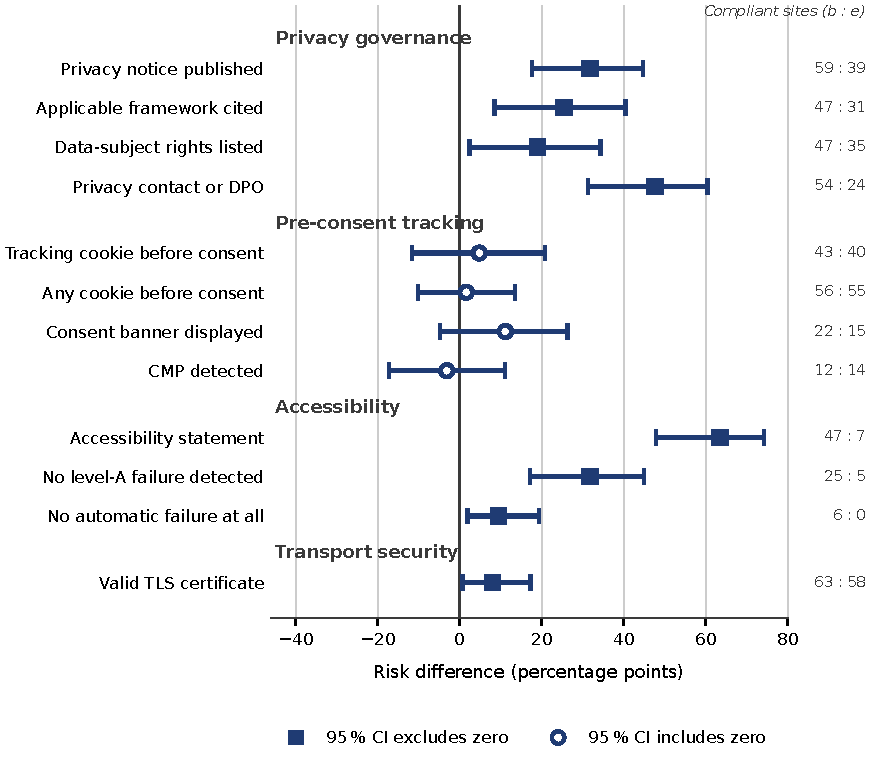
\includegraphics[width=\textwidth]{fig_forest.pdf}
	\caption{Diferencias de riesgo entre el grupo de referencia y el censo ecuatoriano, con intervalos de Newcombe al 95\,\%, agrupadas por dominio. Los cuadrados llenos marcan intervalos que excluyen el cero; los c\'irculos vac\'ios, los que lo incluyen. A la derecha constan los recuentos de sitios que cumplen, sobre 63, en el orden referencia:Ecuador. Los valores positivos indican una proporci\'on mayor en el grupo de referencia.}\label{fig:forest}
\end{figure}

\subsection{Gobernanza de la privacidad (PI1)}\label{sec:results-governance}

Las diferencias de gobernanza fueron las mayores y las m\'as robustas del estudio. Un aviso de privacidad era alcanzable desde la portada en 59 de los 63 sitios de referencia (93,7\,\%) y en 39 de los 63 ecuatorianos (61,9\,\%), una diferencia de 31,7 puntos porcentuales (raz\'on de momios 9,08; $p$ ajustada $<0{,}001$). Exigir adem\'as que el aviso nombre un instrumento legal espec\'ifico redujo ambas cifras, al 74,6\,\% y al 49,2\,\% respectivamente (raz\'on de momios 3,03; $p$ ajustada $=0{,}045$).

La brecha m\'as ancha estuvo en la v\'ia por la que un titular puede actuar. Un canal de contacto o delegado de protecci\'on de datos constaba en el 85,7\,\% de los sitios de referencia y en el 38,1\,\% de los ecuatorianos, una diferencia de 47,6 puntos porcentuales (raz\'on de momios 9,75; $p$ ajustada $<0{,}001$). La enumeraci\'on de derechos difiri\'o en el mismo sentido, 74,6\,\% frente a 55,6\,\%, pero esta diferencia no sobrevivi\'o a la correcci\'on por comparaciones m\'ultiples ($p$ ajustada $=0{,}235$) y aqu\'i se informa \'unicamente como indicio.

El desglose regional del grupo de referencia consta en el Cuadro~\ref{tab:reg}. Debe leerse como descriptivo: con subgrupos de tres a cinco instituciones, el intervalo de Wilson en torno a una proporci\'on abarca m\'as de 50 puntos porcentuales, de modo que estos datos no sostienen ninguna ordenaci\'on regional. Dos patrones merecen, aun as\'i, registro por su magnitud relativa a esa incertidumbre. Las instituciones chinas del grupo son las menos propensas a publicar un aviso de primer nivel, dos de seis, y ninguna publica declaraci\'on de accesibilidad. Europa continental cita un marco legal en nueve de sus diez instituciones, pero esas diez no son homog\'eneas en el instrumento aplicable: dos son suizas y est\'an sujetas a la ley federal de protecci\'on de datos revisada \citep{fadp_ch} y no al RGPD. De igual modo, las tres instituciones canadienses son entidades p\'ublicas regidas por estatutos provinciales del sector p\'ublico \citep{fippa_on,fippa_bc,quebec_privacy} y no por la PIPEDA federal \citep{pipeda2000}, que rige la actividad comercial; se corrige aqu\'i la pr\'actica anterior de describir un r\'egimen canadiense \'unico.

\begin{table}[htbp]
	\centering
	\caption{Grupo de referencia por regi\'on: instituciones que cumplen cada indicador documental sobre el total regional. Se omiten deliberadamente los porcentajes y los intervalos: con $n$ entre 3 y 24 sugerir\'ian una precisi\'on que los datos no tienen.}\label{tab:reg}
	\small
	\begin{tabular}{@{}lccccc@{}}
		\toprule
		\textbf{Regi\'on} & \textbf{$n$} & \textbf{Aviso} & \textbf{Marco} & \textbf{Contacto} & \textbf{Accesib.} \\
		\midrule
		Estados Unidos & 24 & 24 & 17 & 23 & 22 \\
		Reino Unido & 7 & 7 & 4 & 5 & 7 \\
		Europa continental & 10 & 10 & 9 & 10 & 8 \\
		China & 6 & 2 & 2 & 3 & 0 \\
		Hong Kong & 3 & 3 & 3 & 2 & 3 \\
		Resto de Asia & 5 & 5 & 4 & 4 & 0 \\
		Australia & 5 & 5 & 5 & 4 & 4 \\
		Canad\'a & 3 & 3 & 3 & 3 & 3 \\
		\midrule
		\textbf{Total} & \textbf{63} & \textbf{59} & \textbf{47} & \textbf{54} & \textbf{47} \\
		\bottomrule
	\end{tabular}
\end{table}

\subsection{Conducta previa al consentimiento (PI2)}\label{sec:results-cookies}

La Figura~\ref{fig:cookies} recoge las mediciones en vivo. Observados desde el Ecuador, ambos grupos se comportaron de forma semejante. Al menos una cookie se deposit\'o antes de toda interacci\'on con el consentimiento en el 88,9\,\% de los sitios de referencia y en el 87,3\,\% de los ecuatorianos; cookies de rastreo en concreto, en el 68,3\,\% y el 63,5\,\%. La diferencia en el indicador de rastreo fue de 4,8 puntos porcentuales a favor del Ecuador, con un intervalo al 95\,\% de $[-11{,}6, +20{,}7]$ puntos y una $p$ ajustada de 1,000. Un banner visible fue, en ambos grupos, un fen\'omeno minoritario (34,9\,\% y 23,8\,\%), y se detect\'o una plataforma de gesti\'on del consentimiento algo m\'as a menudo en el Ecuador (22,2\,\%) que en el grupo de referencia (19,0\,\%), diferencia bien dentro de la variaci\'on muestral.

\begin{figure}[htbp]
	\centering
	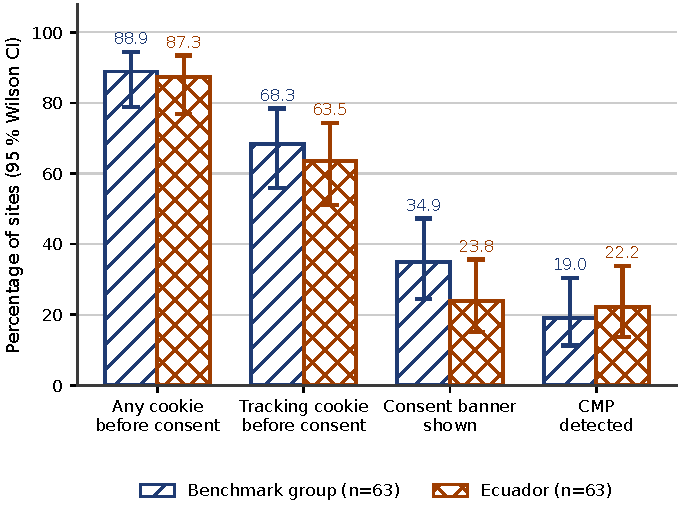
\includegraphics[width=\textwidth]{fig_cookies.pdf}
	\caption{Estado de las cookies registrado antes de toda interacci\'on con una interfaz de consentimiento, con intervalos de Wilson al 95\,\%. Todas las mediciones se tomaron desde un \'unico punto de observaci\'on en el Ecuador en agosto de 2026; un visitante europeo no observar\'ia necesariamente el mismo comportamiento en los sitios europeos del grupo de referencia.}\label{fig:cookies}
\end{figure}

La ausencia de una diferencia detectable no debe leerse como demostraci\'on de equivalencia. Con 63 sitios por grupo y proporciones cercanas a 0,65, la menor diferencia que este dise\~no podr\'ia detectar con una potencia del 80\,\% y $\alpha=0{,}05$ es de unos 24 puntos porcentuales; detectar una diferencia real de 5 puntos exigir\'ia alrededor de 1400 sitios por grupo. Dos pruebas unilaterales lo confirman de forma directa: la equivalencia se rechaza con un margen de $\pm 10$ puntos porcentuales ($p=0{,}267$) y con $\pm 15$ ($p=0{,}113$), y solo se sostiene con un margen de $\pm 20$ ($p=0{,}036$), demasiado ancho para resultar sustantivamente interesante. Demostrar equivalencia dentro de $\pm 10$ puntos exigir\'ia unos 280 sitios por grupo. El enunciado correcto de este resultado es, por tanto, que \emph{el estudio no encontr\'o evidencia de diferencia en el rastreo previo al consentimiento y no tuvo potencia para establecer que los grupos sean equivalentes}.

Una salvedad adicional, y m\'as importante, concierne a lo que un resultado nulo puede significar aqu\'i. Como todas las observaciones se tomaron desde el Ecuador, la cifra del grupo de referencia confunde dos posibilidades de lectura jur\'idica opuesta: que las instituciones europeas no condicionen sus interfaces de consentimiento a la ubicaci\'on del visitante y rastreen a todo el mundo por igual, o que s\'i las condicionen y muestren por tanto a un visitante europeo una interfaz distinta de la registrada aqu\'i. El dise\~no presente no puede distinguirlas, y la Secci\'on~\ref{sec:discussion} expone por qu\'e la distinci\'on importa y c\'omo deber\'ia resolverse.

\subsection{Accesibilidad declarada y seguridad del transporte (PI3, primera parte)}\label{sec:results-declared}

Publicaban una declaraci\'on de accesibilidad o un conjunto de herramientas de accesibilidad 47 de las 63 instituciones de referencia (74,6\,\%) y 7 de las 63 ecuatorianas (11,1\,\%), la mayor diferencia individual del estudio (raz\'on de momios 23,50; $p$ ajustada $<0{,}001$). Deberes legales concretos explican de forma plausible parte de esa brecha: 22 de las 24 instituciones estadounidenses publican una declaraci\'on, en una jurisdicci\'on con la ADA y la Secci\'on 508 \citep{ada1990,section508}, y 8 de las 10 de Europa continental lo hacen bajo la \emph{European Accessibility Act} \citep{eaa2019}. La cifra ecuatoriana es coherente con el rezago regional documentado en la \'ultima d\'ecada \citep{campoverdemolina2023accessibility,acostavargas2020dataset}.

La seguridad del transporte fue casi universal en ambos grupos: hab\'ia un certificado TLS v\'alido en los 63 sitios de referencia y en 58 de los 63 ecuatorianos (92,1\,\%; $p$ ajustada $=0{,}288$). Conviene insistir en que este indicador mide \'unicamente la confidencialidad en tr\'ansito. Un sitio con una cadena de certificados impecable puede transmitir datos del visitante a cualquier n\'umero de terceros, y cinco de los doce indicadores del Cuadro~\ref{tab:comp} muestran precisamente ese patr\'on.

La secci\'on de transparencia LOTAIP exigida a las entidades p\'ublicas ecuatorianas constaba en 47 de las 63 instituciones ecuatorianas (74,6\,\%). Se informa por completitud, porque figura en el Anexo~\ref{ap:ecuador}, y no se emplea en ninguna comparaci\'on, ya que carece de contrapartida en el grupo de referencia.

\subsection{Conformidad WCAG medida (PI3, segunda parte)}\label{sec:results-wcag}

El Cuadro~\ref{tab:wcag} recoge los resultados de la auditor\'ia y la Figura~\ref{fig:wcag} la distribuci\'on de los nodos con fallo por nivel de conformidad.

\begin{table}[htbp]
	\centering
	\caption{Resultados WCAG detectables autom\'aticamente (axe-core 4.13, agosto de 2026, solo portada). Los porcentajes son de sitios salvo indicaci\'on. El conjunto de reglas se especifica en la Secci\'on~\ref{sec:methods-audit}.}\label{tab:wcag}
	\small
	\begin{tabular}{@{}p{7.4cm}cc@{}}
		\toprule
		\textbf{Medida} & \textbf{Referencia} & \textbf{Ecuador} \\
		\midrule
		Mediana de reglas distintas incumplidas por sitio & 2 & 4 \\
		Sitios sin fallo autom\'atico en ning\'un nivel & 9,5\,\% & 0,0\,\% \\
		Sitios sin fallo autom\'atico de nivel A & 39,7\,\% & 7,9\,\% \\
		Enlaces sin nombre accesible (2.4.4, nivel A) & 23,8\,\% & 81,0\,\% \\
		Contraste insuficiente (1.4.3, nivel AA) & 25,4\,\% & 79,4\,\% \\
		Im\'agenes sin alternativa textual (1.1.1, nivel A) & 15,9\,\% & 30,2\,\% \\
		\midrule
		\multicolumn{3}{@{}l}{\textit{Distribuci\'on de nodos con fallo por nivel, con todas las reglas activas}}\\
		\quad Nivel A & 19\,\% & 45\,\% \\
		\quad Nivel AA & 22\,\% & 29\,\% \\
		\quad Nivel AAA & 60\,\% & 26\,\% \\
		\multicolumn{3}{@{}l}{\textit{Misma distribuci\'on excluyendo las reglas AAA y renormalizando}}\\
		\quad Nivel A & 46,3\,\% & 60,8\,\% \\
		\quad Nivel AA & 53,7\,\% & 39,2\,\% \\
		\bottomrule
	\end{tabular}
	\par\vspace{3pt}
	\footnotesize\RaggedRight\textit{Nota:} la mediana es de reglas distintas incumplidas, no de nodos con fallo. Los porcentajes por nivel son del total de nodos con fallo de cada grupo y est\'an redondeados al entero m\'as pr\'oximo, raz\'on por la cual la distribuci\'on del grupo de referencia suma 101\,\%.
\end{table}

\begin{figure}[htbp]
	\centering
	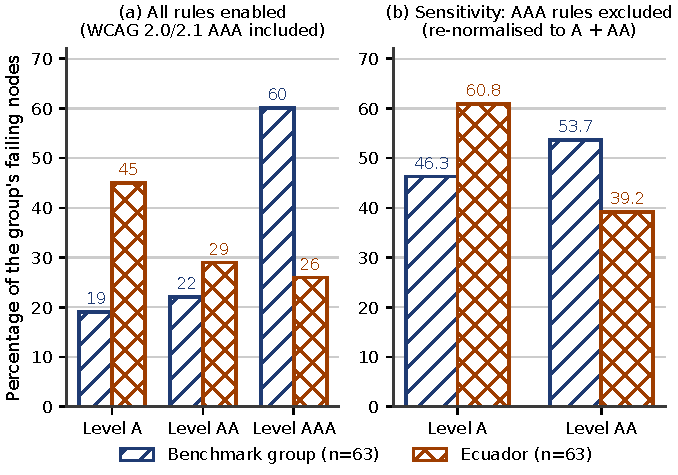
\includegraphics[width=\textwidth]{fig_wcag_niveles.pdf}
	\caption{Distribuci\'on de los nodos con fallo por nivel de conformidad WCAG. El panel (a) emplea el conjunto de reglas completo de este estudio, que incluye las reglas de nivel AAA de WCAG 2.0 y 2.1. El panel (b) las excluye y renormaliza sobre los niveles A y AA, y muestra que la ordenaci\'on de ambos grupos en el nivel A se mantiene cuando no se cuenta la regla de contraste realzado.}\label{fig:wcag}
\end{figure}

Ninguno de los dos grupos obtuvo un buen resultado. Ning\'un sitio ecuatoriano y solo el 9,5\,\% de los de referencia no produjeron fallo autom\'atico alguno en ning\'un nivel activado, y la mediana de reglas distintas incumplidas fue de cuatro en el Ecuador frente a dos en el grupo de referencia. La distinci\'on relevante, sin embargo, es d\'onde caen los fallos. En el grupo de referencia, el 19\,\% de los nodos con fallo correspondi\'o al nivel A y el 60\,\% al nivel AAA, este \'ultimo dominado por el contraste realzado; en el Ecuador, el 45\,\% correspondi\'o al nivel A. Excluir por completo las reglas AAA y renormalizar sobre los niveles A y AA mantiene la ordenaci\'on, 46,3\,\% frente a 60,8\,\% en el nivel A, lo que indica que el hallazgo cualitativo no es un artefacto de haber activado una \'unica regla exigente.

Se corrigen aqu\'i dos afirmaciones que aparec\'ian en una versi\'on anterior de este trabajo, porque los datos no las sostienen. \emph{No} es cierto que ninguna instituci\'on quede libre de fallos autom\'aticos: seis instituciones de referencia lo estuvieron. Y \emph{no} es cierto que el grupo de referencia falle solo en el nivel de excelencia: el 60,3\,\% de sus sitios produjo al menos un fallo de nivel A, de modo que la mayor\'ia del grupo de referencia tampoco supera el umbral b\'asico. Lo que los datos sostienen es m\'as estrecho y sigue mereciendo informe: ambos grupos difieren en la \emph{distribuci\'on} de sus fallos, no en la presencia de fallos.

El caso m\'as claro es el criterio de \'exito 2.4.4, que exige que cada enlace tenga un texto que un lector de pantalla pueda anunciar; lo incumpli\'o el 81,0\,\% de los sitios ecuatorianos y el 23,8\,\% de los de referencia. El contraste insuficiente (1.4.3) sigui\'o el mismo patr\'on, 79,4\,\% frente a 25,4\,\%. El principio m\'as afectado en ambos grupos es el perceptible, por el contraste; el Ecuador suma un d\'eficit operable, por enlaces y controles, marginal en el grupo de referencia. Son los mismos tipos de error dominantes que se informan para otros portales p\'ublicos \citep{iniesto2025service,aljedaani2025egovernment}.

Dos cautelas se aplican a las medidas basadas en niveles. Primera, la distribuci\'on de la Figura~\ref{fig:wcag}(a) se calcula sobre \emph{nodos} con fallo, que no son independientes dentro de un sitio: una sola plantilla con varios miles de elementos de bajo contraste puede dominar la distribuci\'on de su grupo. Segunda, la distribuci\'on es composicional, de modo que un grupo con m\'as fallos de nivel A debe mostrar, por pura aritm\'etica, una cuota AAA menor. Ambas razones aconsejan tratar la distribuci\'on por nivel como descriptiva; las medidas por sitio de la mitad superior del Cuadro~\ref{tab:wcag} son las inferencialmente seguras, y apuntan en el mismo sentido.

\subsection{¿Coinciden los dos compromisos? (PI4)}\label{sec:results-joint}

Sobre los 126 sitios, la correlaci\'on de Spearman entre el volumen de fallos de accesibilidad y el n\'umero de cookies de rastreo es de 0,04. Ese coeficiente tiene un intervalo de confianza al 95\,\% de $[-0{,}14, +0{,}21]$ y $p=0{,}657$, y el dise\~no solo habr\'ia podido detectar una correlaci\'on de alrededor de 0,25 con una potencia del 80\,\%. El coeficiente agrupado es, por tanto, compatible tanto con la ausencia de asociaci\'on como con una asociaci\'on positiva d\'ebil, y no puede sostener una afirmaci\'on de independencia.

El coeficiente agrupado es adem\'as el estimando equivocado, porque mezcla dos poblaciones cuyas distribuciones marginales difieren en ambas variables. El Cuadro~\ref{tab:joint} recoge la clasificaci\'on cruzada, dentro de cada grupo, de las dos medidas dicotomizadas. En el grupo de referencia la asociaci\'on es, si acaso, ligeramente negativa (raz\'on de momios 0,54; $p$ de Fisher $=0{,}408$); en el ecuatoriano es pr\'acticamente nula (raz\'on de momios 1,17; $p$ de Fisher $=1{,}000$); la estimaci\'on de Mantel--Haenszel ajustada por grupo es 0,66. Ninguna es distinguible de la ausencia de asociaci\'on con este tama\~no de muestra.

\begin{table}[htbp]
	\centering
	\caption{Clasificaci\'on cruzada de la conformidad de nivel A detectable autom\'aticamente frente al rastreo previo al consentimiento, dentro de cada grupo. RM: raz\'on de momios de la conformidad dada la contenci\'on en el rastreo, con intervalo al 95\,\%.}\label{tab:joint}
	\small
	\begin{tabular}{@{}lcccccc@{}}
		\toprule
		\textbf{Grupo} & $A^{+}T^{-}$ & $A^{+}T^{+}$ & $A^{-}T^{-}$ & $A^{-}T^{+}$ & \textbf{RM [IC 95\,\%]} & \textbf{$p$} \\
		\midrule
		Referencia & 6 & 19 & 14 & 24 & 0,54 [0,17, 1,68] & 0,408 \\
		Ecuador & 2 & 3 & 21 & 37 & 1,17 [0,18, 7,60] & 1,000 \\
		\bottomrule
	\end{tabular}
	\par\vspace{3pt}
	\footnotesize\RaggedRight\textit{Nota:} $A^{+}$ sin fallo de nivel A detectable autom\'aticamente, $A^{-}$ al menos uno; $T^{-}$ sin cookie de rastreo antes del consentimiento, $T^{+}$ al menos una. El valor $p$ procede de la prueba exacta de Fisher bilateral. En el Ecuador, 2 instituciones de 63 cumplieron ambos criterios; bajo independencia se esperar\'ian $63 \times 0{,}079 \times 0{,}365 \approx 1{,}8$, de modo que esa cifra es exactamente lo que predice el azar y no informa sobre acoplamiento alguno.
\end{table}

La conclusi\'on defendible de la PI4 es negativa, y conviene enunciarla con precisi\'on justamente porque la tentaci\'on es sobreafirmarla. Estos datos no aportan evidencia de que las instituciones que invierten en accesibilidad contengan tambi\'en el rastreo, ni evidencia de lo contrario. No bastan para establecer que ambas sean independientes; establecerlo exigir\'ia una muestra sustancialmente mayor o un par de medidas continuas con mejor potencia.

\subsection{¿Qui\'en determina la protecci\'on? (PI5)}\label{sec:results-vantage}

La replicaci\'on desde cuatro puntos dej\'o 121 de los 126 sitios medidos con \'exito en las tres pasadas de los cuatro puntos. Los tres controles se comportaron como se requer\'ia: la media de violaciones WCAG por sitio fue de 3,53, 3,51, 3,54 y 3,50 en los puntos ecuatoriano, alem\'an, brit\'anico y estadounidense, una dispersi\'on del 1,1\,\%, lo que confirma que las p\'aginas se renderizaron igual. La estabilidad entre pasadas del indicador de rastreo fue del 94,4\,\% al 100\,\%, de modo que tres pasadas bastaron.

El rastreo previo al consentimiento, en cambio, s\'i vari\'o con la ubicaci\'on del visitante. Se observ\'o en el 67,8\,\% de los sitios desde el Ecuador (IC 95\,\% 59,0--75,4), el 65,3\,\% desde los Estados Unidos, el 62,8\,\% desde el Reino Unido y el 60,3\,\% desde Alemania (51,4--68,6). La $Q$ de Cochran sobre los cuatro puntos da $Q=15{,}88$, 3 gl, $p=0{,}0012$. Las comparaciones pareadas del Cuadro~\ref{tab:vantage} localizan la diferencia: el Ecuador difiere de Alemania (9 pares discordantes, todos en el mismo sentido, $p=0{,}0039$) y del Reino Unido ($p=0{,}031$), mientras que el Ecuador y los Estados Unidos son indistinguibles ($p=0{,}25$), igual que el Reino Unido y Alemania ($p=0{,}25$).

\begin{table}[htbp]
	\centering
	\caption{Pruebas exactas de McNemar para el rastreo previo al consentimiento entre puntos de observaci\'on ($n=121$ sitios observados en los cuatro). $b$: sitios que rastrean en el primer punto y no en el segundo; $c$: lo contrario. Solo los pares discordantes aportan informaci\'on.}\label{tab:vantage}
	\small
	\begin{tabular}{@{}lccccc@{}}
		\toprule
		\textbf{Comparaci\'on} & $a$ & $b$ & $c$ & \textbf{Discord.} & \textbf{$p$} \\
		\midrule
		Ecuador vs Alemania & 74 & 9 & 0 & 9 & 0,0039 \\
		Ecuador vs Reino Unido & 77 & 6 & 0 & 6 & 0,031 \\
		Estados Unidos vs Alemania & 73 & 7 & 1 & 8 & 0,070 \\
		Estados Unidos vs Reino Unido & 76 & 4 & 1 & 5 & 0,375 \\
		Reino Unido vs Alemania & 74 & 3 & 0 & 3 & 0,250 \\
		Ecuador vs Estados Unidos & 80 & 3 & 0 & 3 & 0,250 \\
		\bottomrule
	\end{tabular}
\end{table}

El mecanismo se ve al atribuir cada cookie al proveedor que la deposita. La Figura~\ref{fig:vantage} muestra la proporci\'on de sitios en que cada proveedor deposit\'o al menos una cookie antes de toda interacci\'on con el consentimiento. Tres proveedores retuvieron por completo sus cookies ante visitantes europeos y brit\'anicos y las depositaron ante ecuatorianos y estadounidenses en las mismas p\'aginas: Microsoft, cuyas cookies de Clarity, publicidad y UET aparecieron en 14 sitios desde el Ecuador y 14 desde los Estados Unidos y en ninguno desde Alemania o el Reino Unido; TapAd, 4 y 4 frente a cero; y StackAdapt, 2 y 2 frente a cero. El Insight Tag de LinkedIn sigui\'o el mismo patr\'on atenuado, 14 y 14 frente a 3 y 7. Google Analytics, Meta y Adobe redujeron su huella solo de forma moderada y de manera parecida en los cuatro puntos.

\begin{figure}[htbp]
	\centering
	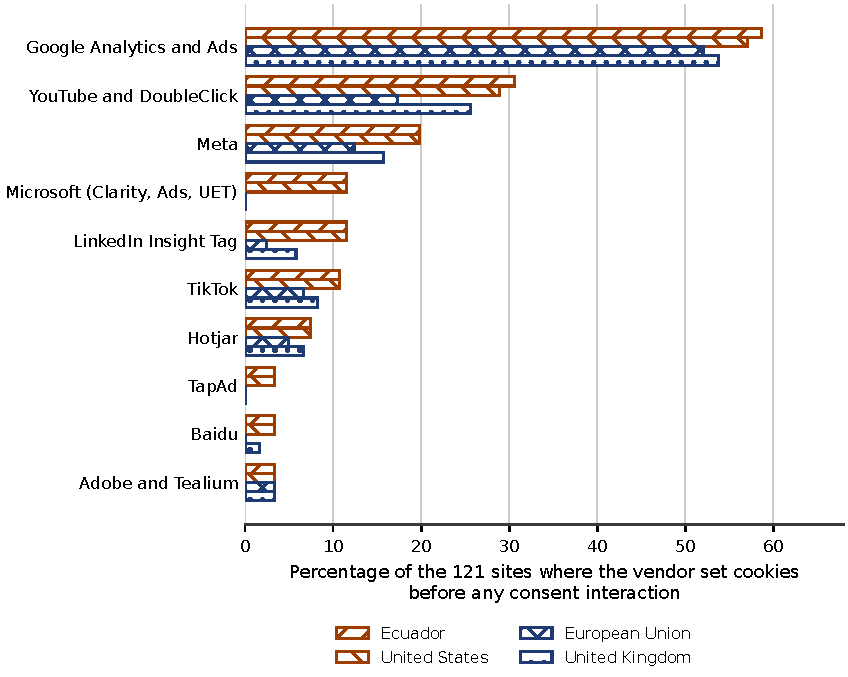
\includegraphics[width=\textwidth]{fig_vantage.pdf}
	\caption{Proporci\'on de sitios en que cada proveedor publicitario deposit\'o al menos una cookie antes de toda interacci\'on con el consentimiento, por punto de observaci\'on ($n=121$ sitios, mayor\'ia de tres pasadas, agosto de 2026). El ocre marca los dos puntos situados fuera del Espacio Econ\'omico Europeo y el azul los dos que quedan dentro del per\'imetro que aplican los proveedores. Se omiten los proveedores presentes en menos de cuatro sitios.}\label{fig:vantage}
\end{figure}

Dos rasgos del patr\'on merecen \'enfasis porque no son los que predice el encuadre institucional. Primero, la supresi\'on no se limita a las instituciones europeas: universidades ecuatorianas, chinas y estadounidenses que incrustan esas etiquetas tambi\'en dejan de depositar las cookies correspondientes cuando el visitante est\'a en Alemania o el Reino Unido. La conducta pertenece, por tanto, al proveedor, no a la instituci\'on ni a la ley que la obliga. Segundo, la mayor\'ia de proveedores trata al Reino Unido como parte del per\'imetro protegido pese a que ya no pertenece al Espacio Econ\'omico Europeo, lo que resulta coherente con que operen una lista de pa\'ises y no una prueba jur\'idica. TikTok y Baidu son la excepci\'on: ambos depositan bastantes m\'as cookies ante visitantes brit\'anicos que ante alemanes, 10 frente a 8 sitios y 2 frente a 0 respectivamente, de modo que el per\'imetro es propio de cada proveedor y no com\'un.

Cabe una salvedad. Las cookies no atribuibles a ning\'un proveedor publicitario tambi\'en descendieron en los puntos europeo y brit\'anico, un 25,8\,\% y un 21,4\,\% frente al Ecuador, mientras que el punto estadounidense difiri\'o solo un 0,8\,\%. Ese residuo es menor que la ca\'ida del 43,6\,\% y el 37,4\,\% en las cookies de proveedor y no afecta a los controles de renderizado, pero es probable que parte de \'el corresponda a la cookie de gesti\'on de robots de Cloudflare y a las que depositan las propias plataformas de consentimiento, cuyo comportamiento tambi\'en var\'ia con la regi\'on del visitante. Se informa aqu\'i en lugar de ajustarlo.

% =============================================================================
\section{Discusi\'on}\label{sec:discussion}
% =============================================================================

\subsection{Interpretaci\'on}\label{sec:discussion-interp}

Tres hallazgos sobreviven al an\'alisis de la Secci\'on~\ref{sec:results}, y son de naturaleza distinta.

El primero es una brecha de gobernanza amplia, robusta a la correcci\'on por comparaciones m\'ultiples y consistente en cuatro indicadores. La carencia ecuatoriana no es principalmente la ausencia de documentos, sino la de los elementos que hacen accionable un documento: un instrumento nombrado, una enumeraci\'on de derechos y, sobre todo, una v\'ia identificada por la que una persona pueda ejercerlos. Los 47,6 puntos de diferencia en el canal de contacto son la cifra de mayor consecuencia del estudio, porque un derecho sin canal no es ejercitable. Que las instituciones de referencia cumplan bien aqu\'i no acredita una \'etica superior; es la consecuencia esperable de reg\'imenes legales que imponen el deber de forma expresa, y sugiere que lo mismo es alcanzable en el Ecuador a medida que la LOPDP y su reglamento entren en su fase de aplicaci\'on \citep{lopdp2021,reglamentolopdp2023}.

El segundo es una brecha de accesibilidad cuya propiedad interesante es su forma. Ambos grupos fallan; la mayor\'ia del grupo de referencia falla tambi\'en en el umbral b\'asico. Lo que difiere es que los fallos ecuatorianos se concentran en el nivel A, donde los remedios son baratos y bien conocidos, principalmente el texto accesible de los enlaces y un contraste suficiente, y donde las consecuencias para quien usa tecnolog\'ia de apoyo son m\'as graves. Es el hallazgo m\'as inmediatamente accionable del estudio y el \'unico que no requiere legislaci\'on nueva para actuar.

El tercero es un resultado nulo sobre el rastreo previo al consentimiento que debe informarse como tal. Observados desde el Ecuador, alrededor de dos tercios de las instituciones de ambos grupos depositaron cookies de rastreo antes de toda interacci\'on con el consentimiento. El estudio no encontr\'o diferencia; tampoco tuvo potencia para establecer equivalencia, y la Secci\'on~\ref{sec:results-cookies} enuncia la cota de forma expresa. Lo que sobrevive no es, por tanto, ``no hay brecha'', sino ``la brecha, de existir, no es grande, y desde luego no va en el sentido que predecir\'ia la jerarqu\'ia reputacional de ambos grupos''.

\subsection{\'Ambito territorial, y qui\'en lo aplica en realidad}\label{sec:discussion-legal}

Una versi\'on anterior de este trabajo explicaba el comportamiento del grupo de referencia diciendo que la protecci\'on del RGPD se detiene en la frontera comunitaria, de modo que quien consulta desde el Ecuador el portal de una universidad europea queda tan expuesto como en un sitio nacional. Esa explicaci\'on era incorrecta en derecho, y la replicaci\'on multipunto muestra que tambi\'en lo era de hecho, aunque no del modo que supusimos al principio.

Primero el punto jur\'idico. El art\'iculo 3(1) del RGPD se aplica al tratamiento en el contexto de las actividades de un establecimiento del responsable en la Uni\'on \emph{con independencia de que el tratamiento tenga lugar en la Uni\'on o no}, y el Comit\'e Europeo de Protecci\'on de Datos ha confirmado que la ubicaci\'on del interesado es irrelevante para ese apartado \citep{gdpr2016,edpb2019territorial}. Una universidad alemana o francesa que instala cookies de marketing en el navegador de un visitante situado en el Ecuador act\'ua, por tanto, dentro del \'ambito del Reglamento. El art\'iculo 3(2) lo extiende a responsables no establecidos en la Uni\'on que ofrecen bienes o servicios a interesados \emph{que se encuentran en} ella. El punto m\'as estrecho y defendible concierne a otro instrumento: el art\'iculo 5(3) de la Directiva ePrivacy, articulado en torno al equipo terminal del usuario, con la gu\'ia del CEPD sobre su \'ambito t\'ecnico como referencia \citep{eprivacy2002,edpb2024eprivacy}.

La medici\'on muestra despu\'es algo que el encuadre institucional no anticipa. La protecci\'on s\'i var\'ia con la ubicaci\'on del visitante, y de forma sustancial, pero no son las universidades las que var\'ian su comportamiento: son los proveedores publicitarios incrustados en sus p\'aginas. Microsoft, TapAd y StackAdapt no depositan cookie alguna ante un visitante situado en Alemania o el Reino Unido y las depositan con normalidad ante uno situado en el Ecuador o los Estados Unidos, y lo hacen en sitios universitarios ecuatorianos, chinos y estadounidenses con la misma facilidad que en los europeos. La instituci\'on es ajena a esto: incrusta una etiqueta, y la etiqueta decide.

De ah\'i se siguen tres consecuencias que, juntas, son la aportaci\'on m\'as original de este estudio.

La primera es que el cumplimiento se est\'a ejecutando en la capa equivocada. Un deber que el derecho europeo impone al responsable, la universidad, lo descarga en la pr\'actica un encargado que la universidad no configur\'o ni audita, sobre la base de una consulta de geolocalizaci\'on. Eso puede satisfacer la letra de la obligaci\'on ante visitantes europeos y dejar al responsable sin conocimiento alguno de lo que hace su propio sitio.

La segunda es que la frontera es comercial, no jur\'idica. El Reino Unido sali\'o del Espacio Econ\'omico Europeo y aun as\'i la mayor\'ia de proveedores lo mantiene dentro del per\'imetro protegido, mientras que TikTok y Baidu no. La protecci\'on de una persona depende, por tanto, de qu\'e listas de pa\'ises mantengan unas cuantas empresas privadas, listas que no se publican, no est\'an armonizadas ni se someten a la revisi\'on que recibir\'ia un instrumento normativo.

La tercera es distributiva, y es el punto que enlaza este hallazgo con la preocupaci\'on por el acceso universal con que abr\'ia este art\'iculo. La poblaci\'on que no recibe protecci\'on alguna es la situada fuera del per\'imetro de los proveedores, que incluye a todo el conjunto de aspirantes internacionales de Am\'erica Latina, \'Africa y buena parte de Asia. A un aspirante ecuatoriano que consulta las p\'aginas de admisi\'on de una universidad alemana se le rastrea; a un aspirante alem\'an que consulta las de una universidad ecuatoriana, no. La asimetr\'ia va en la direcci\'on que agrava la desigualdad existente, y es invisible para cualquier ejercicio de supervisi\'on realizado desde dentro del per\'imetro, que es donde se sit\'uan los reguladores, los auditores y la mayor\'ia de los investigadores.

\subsection{Implicaciones para la pr\'actica}\label{sec:discussion-practice}

Para las instituciones ecuatorianas, el orden que se desprende de estos resultados es inusualmente claro. La primera acci\'on es identificar en el aviso de primer nivel un canal de privacidad por rol y direcci\'on; es la intervenci\'on m\'as barata de la lista y cierra la mayor brecha. La segunda es nombrar el instrumento aplicable y enumerar los derechos que confiere la LOPDP, junto con el procedimiento para ejercerlos, en sustituci\'on de las referencias gen\'ericas a ``la legislaci\'on aplicable''. La tercera es remediar los fallos de accesibilidad de nivel A, empezando por el texto de los enlaces y el contraste, que juntos suman la mayor\'ia de los nodos de nivel A observados. La cuarta, y la menos urgente seg\'un la evidencia recogida aqu\'i, es la interfaz de consentimiento: a\~nadir un banner sin configurarlo para bloquear antes del consentimiento cambia el indicador medido sin cambiar la exposici\'on de la persona usuaria, una sustituci\'on que la literatura de medici\'on ha documentado repetidamente \citep{sanchezrola2019can,bollinger2022automating} y que los datos presentes no permiten descartar en ninguno de los dos grupos.

Para las instituciones del grupo de referencia, el resultado pertinente es que el 60,3\,\% de ellas produce al menos un fallo de nivel A y que dos tercios depositan cookies de rastreo antes del consentimiento cuando se las observa desde fuera de la Uni\'on. La posici\'on reputacional no acredita desempe\~no ni en accesibilidad ni en privacidad. De la Secci\'on~\ref{sec:results-vantage} se deriva otra implicaci\'on que alcanza a todas las instituciones de ambos grupos: quien prueba su propio sitio desde su propia oficina ve \'unicamente lo que su ubicaci\'on le permite ver. Comprobar qu\'e experimenta un aspirante internacional exige medir desde la regi\'on de ese aspirante, algo que no es dif\'icil ni costoso y que, seg\'un esta evidencia, no se est\'a haciendo.

\subsection{Implicaciones para la pol\'itica p\'ublica}\label{sec:discussion-policy}

Se siguen dos implicaciones para los reguladores. Primera, para la autoridad ecuatoriana de protecci\'on de datos, los indicadores que separan con mayor nitidez a ambos grupos son justamente los verificables a bajo costo desde fuera de la instituci\'on, de modo que una autoevaluaci\'on peri\'odica supervisada contra una matriz publicada es administrativamente viable; el libro de c\'odigos del Anexo~\ref{ap:codebook} se ofrece con ese fin. El riesgo asociado es conocido y conviene anticiparlo: un indicador que se convierte en objetivo se satisface en la superficie, y el banner de cookies es el ejemplo m\'as claro de indicador que puede cumplirse sin cambio alguno de conducta.

Segunda, el patr\'on documentado en la Secci\'on~\ref{sec:results-vantage} concierne a las autoridades de control europeas antes que a las ecuatorianas, y plantea una pregunta que la supervisi\'on tal como se practica hoy no formula. Cuando el cumplimiento del art\'iculo 5(3) por parte de un responsable lo entrega de hecho la l\'ogica de geolocalizaci\'on de un encargado, ese responsable no puede demostrar la responsabilidad proactiva del art\'iculo 5(2) sobre una conducta que ni configur\'o ni observa. Una comprobaci\'on supervisora hecha desde dentro del per\'imetro lo dar\'a por conforme. Proponemos que las auditor\'ias de consentimiento se realicen de forma rutinaria desde fuera del Espacio Econ\'omico Europeo y que las listas de pa\'ises que operan los grandes proveedores de etiquetas se traten como objeto supervisable por derecho propio.

\subsection{Amenazas a la validez}\label{sec:threats}

\emph{Validez de constructo.} El rastreo previo al consentimiento se mide de forma uniforme en once jurisdicciones cuyas obligaciones difieren radicalmente; en los Estados Unidos no existe un deber general de consentimiento previo, y la ley ecuatoriana no incorpora un equivalente del art\'iculo 5(3) de la Directiva ePrivacy. El Anexo~\ref{ap:mapeo} asigna a cada indicador la obligaci\'on concreta, si la hay, de cada jurisdicci\'on, y los resultados de la Secci\'on~\ref{sec:results-cookies} se enuncian como conducta observada y no como hallazgos de cumplimiento. ``Sin fallo de nivel A detectado'' es una afirmaci\'on sobre el subconjunto verificable por m\'aquina y no una afirmaci\'on de conformidad \citep{fischer2025coverage}. La seguridad del transporte se informa aparte de la protecci\'on de datos por la raz\'on dada en la Secci\'on~\ref{sec:results-declared}. La medici\'on basada en cookies tampoco capta \verb|localStorage|, \verb|IndexedDB|, la huella digital, los p\'ixeles sin cookie ni el etiquetado del lado del servidor, de modo que las cifras de rastreo aqu\'i informadas son cotas inferiores.

\emph{Validez interna.} El grupo de referencia es un estrato de \'elite y no una muestra del mundo, de modo que los efectos de recursos y de jurisdicci\'on est\'an plenamente confundidos; no se midi\'o un tercer estrato. No se registraron confusores que s\'i podr\'ian haberse recogido, en particular el presupuesto, la matr\'icula, el idioma del sitio, el gestor de contenidos y el proveedor de alojamiento, y este \'ultimo es una fuente plausible de no independencia dentro del grupo ecuatoriano, donde las plantillas compartidas son frecuentes. El tipo de instituci\'on registrado en el Anexo~\ref{ap:ecuador}, p\'ublica, cofinanciada o autofinanciada, no se analiza aqu\'i.

\emph{Fiabilidad.} La codificaci\'on documental se realiz\'o sin doble codificaci\'on y sin coeficiente de fiabilidad entre codificadores. El subestudio de verificaci\'on de la Secci\'on~\ref{sec:methods-coding} hall\'o dos errores en 24 celdas reexaminadas; no acota nada, pero no es tranquilizador, y la codificaci\'on de \'items que exigen juicio en varios idiomas, entre ellos el chino, el japon\'es, el coreano, el alem\'an, el franc\'es y el sueco, es la parte m\'as expuesta del dise\~no. Los c\'odigos parciales se trataron como incumplimiento, convenci\'on que penaliza a las instituciones con avisos segmentados; los porcentajes no se recalcularon bajo la convenci\'on alternativa. Los c\'odigos de sitios no verificables permanecieron en el denominador, lo que deprime espec\'ificamente los porcentajes ecuatorianos, ya que todos esos casos ocurren en ese grupo.

\emph{Artefactos del punto de observaci\'on.} Los tres puntos no ecuatorianos se alcanzaron mediante una VPN comercial y sus direcciones de salida pertenecen a centros de datos, de modo que un proveedor que tratara esas direcciones de forma distinta podr\'ia, en principio, imitar un efecto de ubicaci\'on. Tres observaciones lo acotan: los controles de renderizado fueron id\'enticos entre puntos hasta un 1,1\,\%; los extremos alem\'an y estadounidense comparten tipo de red, de modo que su contraste queda libre del artefacto; y uno de los extremos alemanes se sustituy\'o por un segundo proveedor en otro sistema aut\'onomo con resultado indistinguible. El descenso residual de cookies ajenas a los proveedores en los puntos europeo y brit\'anico, informado en la Secci\'on~\ref{sec:results-vantage}, no queda explicado del todo y es el punto m\'as d\'ebil de esta parte del dise\~no. Los cuatro puntos se midieron adem\'as en un solo d\'ia, de modo que la replicaci\'on describe la conducta de los proveedores en esa fecha.

\emph{Estabilidad de la medici\'on.} La revisi\'on documental sigue siendo una sola observaci\'on. El estado de cookies previo al consentimiento no es determinista: depende de pruebas A/B, subastas publicitarias, nodo de CDN y momento del despliegue. En la auditor\'ia en vivo esto se abord\'o con las tres pasadas por punto, cuya concordancia entre pasadas fue del 94,4\,\% al 100\,\%; en la comparaci\'on entre grupos de la Secci\'on~\ref{sec:results-cookies}, que descansa en la medici\'on de una sola pasada de agosto, no. Solo se audit\'o la portada, mientras que la conformidad WCAG se define sobre p\'aginas y procesos completos, y las rutas transaccionales que este art\'iculo invoca como motivaci\'on, admisi\'on y matr\'icula, no se midieron. Los detectores de banner y de CMP son heur\'isticos y sus tasas de falsos negativos se desconocen.

\emph{Validez de la conclusi\'on estad\'istica.} Se corrigieron doce comparaciones por el procedimiento de Holm y solo los valores ajustados sostienen afirmaciones; el desglose regional se informa sin inferencia por la raz\'on dada en la Secci\'on~\ref{sec:results-governance}. Los m\'argenes de equivalencia del an\'alisis TOST no fueron preespecificados. La distribuci\'on de accesibilidad por nodos est\'a sujeta a seudorreplicaci\'on y a restricci\'on composicional, como se indica en la Secci\'on~\ref{sec:results-wcag}. Los recuentos de fallos no se normalizaron por complejidad de p\'agina, de modo que un portal extenso acumular\'a m\'as nodos con fallo que uno peque\~no sin ser necesariamente menos accesible.

\emph{Validez externa.} Todas las observaciones se tomaron en una fecha y desde un pa\'is, y los resultados describen el estado de 126 portadas en agosto de 2026. El contenido web cambia; ninguna afirmaci\'on de este art\'iculo debe leerse como una propiedad duradera de instituci\'on alguna.

% =============================================================================
\section{Conclusiones y trabajo futuro}\label{sec:conclusions}
% =============================================================================

Medidas contra un referente de 63 universidades de \'elite, las 63 IES ecuatorianas mostraron sus brechas m\'as amplias y robustas en la gobernanza de la privacidad, sobre todo en la identificaci\'on de un canal de contacto (38,1\,\% frente a 85,7\,\%) y en la publicaci\'on de un aviso de privacidad de primer nivel (61,9\,\% frente a 93,7\,\%). En accesibilidad, ambos grupos fallaron, pero los fallos se distribuyeron de forma distinta: el 45\,\% de los nodos con fallo del Ecuador estaba en el nivel b\'asico A frente al 19\,\% del grupo de referencia, ordenaci\'on que se mantiene al excluir las reglas de nivel AAA. En el rastreo previo al consentimiento, observado desde el Ecuador, el estudio no hall\'o diferencia entre los grupos ni tuvo potencia para establecer que sean equivalentes. Dentro de cada grupo, la accesibilidad medida y la contenci\'on observada en el rastreo no estaban asociadas.

Replicar la auditor\'ia en vivo desde cuatro puntos de observaci\'on estableci\'o despu\'es que la exposici\'on previa al consentimiento la gobierna la ubicaci\'on del visitante y no la de la instituci\'on. Las mismas p\'aginas rastrearon en el 67,8\,\% de los casos ante un visitante ecuatoriano y en el 60,3\,\% ante uno alem\'an ($Q$ de Cochran, $p=0{,}0012$), y la supresi\'on la ejecutaron los proveedores publicitarios: Microsoft, TapAd y StackAdapt no depositaron nada ante visitantes europeos y brit\'anicos mientras rastreaban a los ecuatorianos y estadounidenses en esas mismas p\'aginas, incluidas las de universidades ecuatorianas y chinas.

Estos hallazgos sostienen una conclusi\'on pr\'actica, una jur\'idica y una distributiva. La pr\'actica es que las carencias propias del Ecuador est\'an en la gobernanza y en la accesibilidad de nivel b\'asico, y ambas son remediables sin legislaci\'on nueva. La jur\'idica es que un deber que el derecho europeo impone al responsable lo descargan en la pr\'actica los encargados sobre la base de listas de pa\'ises no publicadas, lo que satisface al visitante de Fr\'ancfort y deja al responsable sin capacidad de demostrar responsabilidad proactiva sobre lo que hace su propio sitio. La distributiva es la que devuelve este art\'iculo a su punto de partida: quienes no reciben protecci\'on son los aspirantes situados fuera del per\'imetro que describen esas listas, es decir, la mayor parte del conjunto internacional de aspirantes, y su exposici\'on es invisible para quien mida desde dentro.

De las amenazas enunciadas en la Secci\'on~\ref{sec:threats} se derivan otros cuatro puntos: doble codificaci\'on independiente de al menos el 30\,\% de la muestra con un $\kappa$ de Cohen por indicador y reconciliaci\'on completa de discrepancias; extensi\'on de la auditor\'ia a un m\'inimo de cinco p\'aginas por sitio, incluida una ruta de admisi\'on o matr\'icula, con la p\'agina como unidad y el sitio como efecto aleatorio; medidas de rastreo m\'as robustas que la cookie, en particular el recuento de dominios de terceros distintos contactados antes del consentimiento; y un an\'alisis interno del grupo ecuatoriano por tipo de instituci\'on, tama\~no y plataforma, para el cual la variable necesaria ya consta en el Anexo~\ref{ap:ecuador} y que probablemente tenga mayor valor local que cualquier comparaci\'on internacional. A ellos los presentes resultados a\~naden un quinto: cartografiar las listas de pa\'ises que operan los grandes proveedores de etiquetas, midiendo desde un punto de observaci\'on por jurisdicci\'on candidata, para describir emp\'iricamente el per\'imetro dentro del cual se entrega la protecci\'on en lugar de suponer que coincide con alguna frontera jur\'idica.

\backmatter

\bmhead{Informaci\'on suplementaria}
El gui\'on de auditor\'ia, su configuraci\'on, la salida cruda por sitio en JSON de las doce pasadas multipunto y los registros de verificaci\'on de ubicaci\'on, el inventario completo de cookies con su clasificaci\'on, la matriz documental, el libro de c\'odigos y los cuadernos de an\'alisis se depositan en un repositorio p\'ublico. \textcolor{gris}{[AUTORES: depositar en Zenodo u OSF antes del env\'io y sustituir por el DOI asignado.]}

\bmhead{Agradecimientos}
\textcolor{gris}{[AUTORES: completar o eliminar.]}

\section*{Declaraciones}

\bmhead{Financiaci\'on}
\textcolor{gris}{[AUTORES: declarar la financiaci\'on recibida o indicar que no se recibi\'o financiaci\'on espec\'ifica.]}

\bmhead{Conflicto de intereses}
El autor de correspondencia y el tercer autor est\'an afiliados a la Universidad T\'ecnica Estatal de Quevedo, una de las 63 instituciones ecuatorianas evaluadas en este estudio y que figura en el Anexo~\ref{ap:ecuador}. La segunda autora est\'a afiliada al Ministerio de Educaci\'on del Ecuador, entidad p\'ublica del mismo sistema educativo nacional. Ninguna de las dos instituciones intervino en el dise\~no del estudio, en la recolecci\'on o codificaci\'on de datos, en el an\'alisis ni en la decisi\'on de publicar. \textcolor{gris}{[AUTORES: si el Ministerio particip\'o de alg\'un modo en dise\~no, financiaci\'on o aprobaci\'on, debe declararse aqu\'i. Se recomienda, adem\'as, que la codificaci\'on de la propia UTEQ sea reproducida por un tercero independiente antes del env\'io.]}

\bmhead{Contribuci\'on de los autores}
\textcolor{gris}{[AUTORES: completar seg\'un la taxonom\'ia CRediT, por ejemplo:]} G.G.-U.: conceptualizaci\'on, metodolog\'ia, software, an\'alisis formal, redacci\'on del borrador original. A.Z.P.: investigaci\'on, curaci\'on de datos, redacci\'on, revisi\'on y edici\'on. E.D.-M.: investigaci\'on, validaci\'on, redacci\'on, revisi\'on y edici\'on. Todos los autores leyeron y aprobaron el manuscrito final.

\bmhead{Disponibilidad de datos}
Los conjuntos de datos generados y analizados durante el estudio est\'an disponibles en el repositorio citado en la informaci\'on suplementaria. \textcolor{gris}{[AUTORES: sustituir por el DOI del dep\'osito.]}

\bmhead{Disponibilidad de c\'odigo}
El gui\'on de auditor\'ia y el c\'odigo de an\'alisis est\'an disponibles en el mismo repositorio.

\bmhead{Aprobaci\'on \'etica y consentimiento}
No aplica. El estudio analiz\'o p\'aginas web de acceso p\'ublico y no involucr\'o participantes humanos, animales ni datos personales.

\bmhead{Uso de inteligencia artificial generativa}
\textcolor{gris}{[AUTORES: declarar si se emple\'o alguna herramienta de IA generativa en la redacci\'on o el an\'alisis y con qu\'e alcance, o indicar expresamente que no se emple\'o.]}

\bmhead{ORCID}
\textcolor{gris}{[AUTORES: a\~nadir los tres identificadores ORCID en el sistema de env\'io de Springer.]}

% =============================================================================
\begin{appendices}
% =============================================================================

\renewcommand{\thetable}{\thesection\arabic{table}}
\renewcommand{\thefigure}{\thesection\arabic{figure}}

\section{Libro de c\'odigos y definiciones operativas}\label{ap:codebook}
\setcounter{table}{0}\setcounter{figure}{0}

El Cuadro~\ref{tab:codebook} recoge la definici\'on operativa, la regla de decisi\'on y el tratamiento de los casos ambiguos de cada indicador. A continuaci\'on consta la taxonom\'ia de cookies de rastreo.

\footnotesize
\begin{longtable}{@{}>{\RaggedRight}p{2.7cm}>{\RaggedRight}p{4.75cm}>{\RaggedRight\arraybackslash}p{4.55cm}@{}}
	\caption{Definiciones operativas de los indicadores codificados.}\label{tab:codebook}\\
	\toprule
	\textbf{Indicador} & \textbf{Se codifica presente cuando} & \textbf{Se codifica ausente o parcial cuando} \\
	\midrule
	\endfirsthead
	\multicolumn{3}{c}{\textit{(Cuadro~\ref{tab:codebook}, continuaci\'on)}}\\
	\toprule
	\textbf{Indicador} & \textbf{Se codifica presente cuando} & \textbf{Se codifica ausente o parcial cuando} \\
	\midrule
	\endhead
	\midrule
	\multicolumn{3}{r}{\textit{Contin\'ua en la siguiente p\'agina}}\\
	\endfoot
	\bottomrule
	\endlastfoot
	Aviso de privacidad & Un documento que describe el tratamiento de datos personales es alcanzable desde la portada o a un clic de ella & \textbf{P} si su \'ambito declarado cubre solo parte del tratamiento institucional; ausente si no es alcanzable desde la portada \\
	\addlinespace
	Marco legal citado & El aviso nombra un instrumento espec\'ifico, por ejemplo la LOPDP, el RGPD o la PDPO & Ausente ante f\'ormulas gen\'ericas como ``la legislaci\'on aplicable''; \textbf{P} si nombra un marco que no le resulta aplicable \\
	\addlinespace
	Derechos enumerados & Se enumeran al menos tres de acceso, rectificaci\'on, supresi\'on, limitaci\'on, oposici\'on y portabilidad, con una v\'ia para ejercerlos & Ausente ante una menci\'on no enumerada de ``sus derechos''; \textbf{P} si se enumeran sin v\'ia alguna \\
	\addlinespace
	Contacto o delegado & Se ofrece un rol nombrado, una direcci\'on o un formulario espec\'ificos para asuntos de privacidad & Ausente ante un formulario institucional general o una centralita \\
	\addlinespace
	Accesibilidad declarada & Se publica una declaraci\'on de accesibilidad, una pol\'itica o una barra de herramientas de accesibilidad & Ausente cuando la accesibilidad solo se menciona dentro de otro documento \\
	\addlinespace
	Seguridad del transporte & La portada se sirve por HTTPS con una cadena que un navegador actual acepta sin advertencia & Ausente ante cadenas caducadas, autofirmadas o incompletas \\
	\addlinespace
	Rastreo previo al consentimiento & Hay al menos una cookie cuyo nombre coincide con la taxonom\'ia siguiente antes de toda interacci\'on con una interfaz de consentimiento & Ausente cuando no hay ninguna cookie coincidente \\
	\addlinespace
	Sin fallo de nivel A & axe-core no informa ninguna violaci\'on con etiqueta de nivel A & Ausente cuando se informa al menos una violaci\'on de nivel A \\
\end{longtable}
\normalsize

\emph{Taxonom\'ia de cookies de rastreo.} Una cookie se clasific\'o como perteneciente a un proveedor publicitario o de anal\'itica cuando su nombre coincid\'ia con alguno de los siguientes patrones, aplicados como expresiones regulares. La lista se ampli\'o tras la replicaci\'on multipunto de la Secci\'on~\ref{sec:methods-vantage}; las familias a\~nadidas entonces van marcadas con asterisco, y todas las cifras del art\'iculo usan la lista ampliada, aplicada reclasificando los nombres almacenados.

\begin{itemize}
	\item \emph{Google Analytics y Ads}: \verb|^_ga|, \verb|^_gid$|, \verb|^__utm|, \verb|^_gcl_|, \verb|^_gac_|; \emph{Privacy Sandbox}*: \verb|^receive-cookie-deprecation$|.
	\item \emph{YouTube y DoubleClick}: \verb|^YSC$|, \verb|^VISITOR_INFO|, \verb|^VISITOR_PRIVACY|*, \verb|^__Secure-YNID$|*, \verb|^__Secure-ROLLOUT|*, \verb|^IDE$|, \verb|^test_cookie$|, \verb|^DSID$|*.
	\item \emph{Meta}: \verb|^_fbp$|, \verb|^_fbc$|, \verb|^fr$|. \emph{TikTok}: \verb|^_tt_|, \verb|^_ttp$|, \verb|^ttcsid|*.
	\item \emph{Microsoft Clarity, Advertising y UET}: \verb|^_clck$|, \verb|^_clsk$|, \verb|^MUID$|, \verb|^MR$|*, \verb|^SM$|*, \verb|^SRM_B$|*, \verb|^ANONCHK$|*, \verb|^CLID$|*, \verb|^_uet|.
	\item \emph{LinkedIn Insight Tag}*: \verb|^bcookie$|, \verb|^bscookie$|, \verb|^lidc$|, \verb|^li_sugr$|, \verb|^li_gc$|, \verb|^UserMatchHistory$|, \verb|^AnalyticsSyncHistory$|.
	\item \emph{TapAd}*: \verb|^TapAd_|. \emph{StackAdapt}*: \verb|^sa-user-id|. \emph{Snapchat}*: \verb|^_scid|, \verb|^sc_at$|.
	\item \emph{X y Twitter}: \verb|^muc_ads$|*, \verb|^personalization_id$|, \verb|^_twpid$|*.
	\item \emph{Hotjar}: \verb|^_hj|. \emph{Siteimprove}: \verb|^nmstat$|. \emph{Matomo}: \verb|^_pk_|. \emph{PixelYourSite y Sourcebuster}: \verb|^pys|, \verb|^sbjs_|*. \emph{Pinterest}: \verb|^_pin_|.
	\item \emph{Adobe y Tealium}: \verb|^AMCV_|, \verb|^s_|, \verb|^utag|, \verb|^mbox|; \emph{ContentSquare}*: \verb|^_cs_|.
	\item \emph{Baidu}: \verb|^Hm_lvt_|, \verb|^Hm_lpvt_|, \verb|^HMACCOUNT|, \verb|^BAIDUID$|. \emph{Quantcast}: \verb|^__qca$|. \emph{LiveIntent}: \verb|^_lc2_|, \verb|^ln_or$|.
\end{itemize}

La lista se basa en nombres y es por tanto conservadora: un proveedor que use un nombre no listado o aleatorizado no se contabiliza, lo que explica en parte que las cifras de la Secci\'on~\ref{sec:results-cookies} sean cotas inferiores. La consecuencia de las omisiones iniciales se cuantifica en la Secci\'on~\ref{sec:results-vantage}: con la lista original la ca\'ida de cookies de proveedor en el punto europeo era del 33,0\,\%, y con la ampliada es del 43,6\,\%.

\section{Mapeo indicador por jurisdicci\'on}\label{ap:mapeo}
\setcounter{table}{0}\setcounter{figure}{0}

El Cuadro~\ref{tab:mapeo} indica, para cada jurisdicci\'on del estudio, el instrumento aceptado como marco aplicable y si la jurisdicci\'on impone un deber general de consentimiento previo para las cookies no esenciales. Es la base de la distinci\'on, mantenida a lo largo de la Secci\'on~\ref{sec:results}, entre conducta observada e incumplimiento legal. La Figura~\ref{fig:cronologia} del Anexo~\ref{ap:figuras} sit\'ua estos reg\'imenes en una cronolog\'ia com\'un.

\footnotesize
\begin{longtable}{@{}>{\RaggedRight}p{2.4cm}>{\RaggedRight}p{5.5cm}>{\RaggedRight\arraybackslash}p{4.1cm}@{}}
	\caption{Marco aplicable y deber de consentimiento previo por jurisdicci\'on.}\label{tab:mapeo}\\
	\toprule
	\textbf{Jurisdicci\'on} & \textbf{Instrumento aceptado como marco aplicable} & \textbf{Deber general de consentimiento previo} \\
	\midrule
	\endfirsthead
	\multicolumn{3}{c}{\textit{(Cuadro~\ref{tab:mapeo}, continuaci\'on)}}\\
	\toprule
	\textbf{Jurisdicci\'on} & \textbf{Instrumento aceptado como marco aplicable} & \textbf{Deber general de consentimiento previo} \\
	\midrule
	\endhead
	\midrule
	\multicolumn{3}{r}{\textit{Contin\'ua en la siguiente p\'agina}}\\
	\endfoot
	\bottomrule
	\endlastfoot
	Ecuador & LOPDP y su reglamento \citep{lopdp2021,reglamentolopdp2023} & Sin equivalente del art.\ 5(3) ePrivacy; el consentimiento se exige para el tratamiento, no como regla de acceso al equipo \\
	\addlinespace
	Uni\'on Europea & RGPD \citep{gdpr2016} y transposiciones nacionales de la Directiva ePrivacy \citep{eprivacy2002} & S\'i, por el art.\ 5(3) ePrivacy seg\'un transposici\'on \citep{edpb2024eprivacy} \\
	\addlinespace
	Reino Unido & UK GDPR y Data Protection Act 2018 \citep{ukdpa2018} & S\'i, por la transposici\'on nacional de ePrivacy \\
	\addlinespace
	Suiza & Ley federal de protecci\'on de datos \citep{fadp_ch} & Sin regla general de consentimiento previo; rigen transparencia y oposici\'on \\
	\addlinespace
	Estados Unidos & CCPA \citep{ccpa2018} para California; FERPA \citep{ferpa1974} e HIPAA \citep{hipaa1996} rigen los expedientes educativos y la informaci\'on sanitaria protegida, no el portal p\'ublico & Sin deber general de consentimiento previo; modelo de exclusi\'on voluntaria \\
	\addlinespace
	Canad\'a & Estatutos provinciales del sector p\'ublico para las universidades p\'ublicas \citep{fippa_on,fippa_bc,quebec_privacy}; PIPEDA \citep{pipeda2000} para la actividad comercial & Sin deber general de consentimiento previo; se reconoce el consentimiento impl\'icito \\
	\addlinespace
	China & PIPL \citep{pipl2021} & Consentimiento exigido para el tratamiento no esencial \\
	\addlinespace
	Jap\'on & APPI \citep{appi2003} & Sin deber general de consentimiento previo para las cookies como tales \\
	\addlinespace
	Corea del Sur & PIPA \citep{pipa2011} & Consentimiento exigido para el tratamiento no esencial \\
	\addlinespace
	Singapur & PDPA \citep{pdpa2012} & Modelo de consentimiento presunto; sin deber general previo \\
	\addlinespace
	Australia & Privacy Act 1988 \citep{privacyact1988} & Sin deber general de consentimiento previo \\
	\addlinespace
	Hong Kong & PDPO \citep{pdpo_hk} & Sin deber general de consentimiento previo \\
\end{longtable}
\normalsize

La consecuencia interpretativa es directa: en la mayor\'ia de las jurisdicciones estudiadas, depositar una cookie de rastreo antes del consentimiento no es en s\'i mismo il\'icito. El indicador se conserva porque mide la exposici\'on del visitante, que es la preocupaci\'on de este art\'iculo, pero no es, ni en ning\'un lugar se presenta como, una tasa de cumplimiento.

\section{Matriz documental del grupo de referencia}\label{ap:mundo}
\setcounter{table}{0}\setcounter{figure}{0}

Leyenda: \si{} presente; \no{} ausente; \textbf{P} parcial, es decir, \'ambito acotado o marco gen\'erico; \nv{} no verificable por este m\'etodo. Rankings: QS 2026, THE 2026 y ARWU 2025, con la posici\'on y ``--'' para la ausencia del \emph{top} 75 de ese ranking. Pa\'is en c\'odigo ISO 3166-1 alfa-2. Columnas: Avi.\ (aviso de privacidad de primer nivel), Mar.\ (instrumento legal espec\'ifico nombrado), Der.\ (derechos del titular enumerados), DPO (canal de contacto o delegado identificado), Ckp.\ (se publica una pol\'itica de cookies espec\'ifica, indicador documental distinto de la medici\'on en vivo del banner de la Secci\'on~\ref{sec:results-cookies}), Acc.\ (declaraci\'on o herramientas de accesibilidad). Fecha de codificaci\'on: agosto de 2026. Las celdas marcadas con $\dagger$ se corrigieron tras la reverificaci\'on manual descrita en la Secci\'on~\ref{sec:methods-coding}.

\scriptsize
\setlength{\tabcolsep}{2.6pt}
\begin{longtable}{@{}r l c c c c c c c c c c@{}}
	\caption{Matriz documental de las 63 instituciones de referencia.}\label{tab:mundo}\\
	\toprule
	\textbf{\#} & \textbf{Sigla} & \textbf{P} & \textbf{QS} & \textbf{THE} & \textbf{ARWU} & \textbf{Avi.} & \textbf{Mar.} & \textbf{Der.} & \textbf{DPO} & \textbf{Ckp.} & \textbf{Acc.} \\
	\midrule
	\endfirsthead
	\multicolumn{12}{c}{\textit{(Cuadro~\ref{tab:mundo}, continuaci\'on)}}\\
	\toprule
	\textbf{\#} & \textbf{Sigla} & \textbf{P} & \textbf{QS} & \textbf{THE} & \textbf{ARWU} & \textbf{Avi.} & \textbf{Mar.} & \textbf{Der.} & \textbf{DPO} & \textbf{Ckp.} & \textbf{Acc.} \\
	\midrule
	\endhead
	\midrule
	\multicolumn{12}{r}{\textit{Contin\'ua en la siguiente p\'agina}}\\
	\endfoot
	\bottomrule
	\endlastfoot
	1 & MIT & US & 1 & 2 & 3 & \si & \si & \si & \si & \no & \si \\
	2 & Stanford & US & 3 & 5 & 2 & \si & \si & \si & \si & \si & \si \\
	3 & Harvard & US & 5 & 5 & 1 & \si & \no$^\dagger$ & \no & \no & \no & \si \\
	4 & Oxford & GB & 4 & 1 & 6 & \si & \si & \si & \si & \si & \si \\
	5 & Cambridge & GB & 6 & 3 & 4 & \si$^\dagger$ & \pc & \no & \no & \si & \si \\
	6 & Caltech & US & 10 & 7 & 9 & \si & \si & \no & \si & \no & \si \\
	7 & UC Berkeley & US & 17 & 9 & 5 & \si & \si & \no & \si & \no & \si \\
	8 & Princeton & US & 25 & 3 & 7 & \si & \si & \si & \si & \no & \si \\
	9 & Imperial & GB & 2 & 8 & 26 & \si & \si & \pc & \no & \si & \si \\
	10 & U Chicago & US & 13 & 15 & 10 & \si & \pc & \si & \si & \no & \no \\
	11 & ETH Zurich & CH & 7 & 11 & 22 & \si & \si & \si & \si & \no & \si \\
	12 & Yale & US & 21 & 10 & 11 & \si & \si & \pc & \si & \no & \si \\
	13 & UPenn & US & 15 & 14 & 14 & \si & \pc & \si & \si & \no & \si \\
	14 & UCL & GB & 9 & 22 & 14 & \si & \pc & \si & \si & \si & \si \\
	15 & Cornell & US & 16 & 18 & 12 & \si & \pc & \si & \si & \no & \si \\
	16 & Tsinghua & CN & 17 & 12 & 18 & \si & \si & \si & \si & \no & \no \\
	17 & Peking & CN & 14 & 13 & 23 & \pc & \pc & \no & \no & \no & \no \\
	18 & Johns Hopkins & US & 24 & 16 & 19 & \si & \si & \si & \si & \no & \si \\
	19 & Columbia & US & 38 & 20 & 8 & \si & \si & \si & \si & \si & \si \\
	20 & Toronto & CA & 29 & 21 & 25 & \si & \si & \si & \si & \no & \si \\
	21 & UCLA & US & 46 & 18 & 16 & \si & \si & \si & \si & \no & \si \\
	22 & NUS & SG & 8 & 17 & 56 & \si & \si & \si & \si & \no & \no \\
	23 & U Tokyo & JP & 36 & 26 & 31 & \si & \si & \si & \no & \no & \no \\
	24 & TUM & DE & 22 & 27 & 45 & \si & \si & \si & \si & \no & \no \\
	25 & Melbourne & AU & 19 & 37 & 38 & \si & \si & \si & \si & \no & \no \\
	26 & Edinburgh & GB & 34 & 29 & 37 & \si & \si & \si & \si & \no & \si \\
	27 & EPFL & CH & 22 & 35 & 44 & \si & \si & \si & \si & \no & \si \\
	28 & Michigan & US & 45 & 23 & 33 & \si & \no & \no & \si & \no & \no \\
	29 & Northwestern & US & 42 & 30 & 31 & \si & \pc & \si & \si & \si & \si \\
	30 & Fudan & CN & 30 & 36 & 41 & \no & \no & \no & \no & \no & \no \\
	31 & PSL & FR & 28 & 48 & 34 & \si & \si & \si & \si & \no & \no \\
	32 & HKU & HK & 11 & 33 & 67 & \si & \si & \si & \si & \no & \si \\
	33 & Zhejiang & CN & 49 & 39 & 24 & \si & \pc & \si & \si & \no & \no \\
	34 & NYU & US & 55 & 31 & 28 & \si & \si & \si & \si & \no & \si \\
	35 & SJTU & CN & 47 & 40 & 30 & \no & \no & \no & \no & \no & \no \\
	36 & KCL & GB & 31 & 38 & 61 & \si & \pc & \si & \si & \si & \si \\
	37 & UCSD & US & 66 & 47 & 20 & \si & \si & \si & \si & \no & \si \\
	38 & LMU & DE & 58 & 34 & 42 & \si & \si & \si & \si & \no & \si \\
	39 & Duke & US & 62 & 28 & 46 & \si & \si & \si & \si & \no & \si \\
	40 & Manchester & GB & 35 & 56 & 46 & \si & \si & \pc & \si & \no & \si \\
	41 & UBC & CA & 40 & 45 & 53 & \si & \si & \pc & \si & \no & \si \\
	42 & Sydney & AU & 25 & 53 & 72 & \si & \si & \si & \si & \no & \si \\
	43 & Paris-Saclay & FR & 70 & 68 & 13 & \si & \si & \si & \si & \si & \si \\
	44 & Kyoto & JP & 57 & 61 & 46 & \si & \pc & \si & \si & \no & \no \\
	45 & Illinois & US & 70 & 41 & 53 & \si & \si & \si & \si & \no & \si \\
	46 & UT Austin & US & 68 & 50 & 49 & \si & \si & \si & \si & \no & \si \\
	47 & UW & US & -- & 25 & 17 & \si & \si & \si & \si & \no & \si \\
	48 & NTU & SG & 12 & 31 & -- & \si & \si & \si & \si & \no & \no \\
	49 & McGill & CA & 27 & 41 & -- & \si & \si & \si & \si & \si & \si \\
	50 & CUHK & HK & 32 & 41 & -- & \si & \si & \si & \no & \no & \si \\
	51 & CMU & US & 52 & 24 & -- & \si & \si & \si & \si & \no & \si \\
	52 & Wisconsin & US & -- & 53 & 36 & \si & \si & \no & \si & \si & \si \\
	53 & USTC & CN & -- & 51 & 40 & \pc & \si & \si & \si & \no & \no \\
	54 & WUSTL & US & -- & 67 & 26 & \si & \no & \no & \si & \no & \si \\
	55 & Monash & AU & 36 & 58 & -- & \si & \si & \no & \no & \no & \si \\
	56 & SNU & KR & 38 & 58 & -- & \si & \si & \si & \si & \no & \no \\
	57 & Heidelberg & DE & -- & 49 & 51 & \si & \si & \si & \si & \no & \si \\
	58 & HKUST & HK & 44 & 58 & -- & \si & \si & \si & \si & \no & \si \\
	59 & Karolinska & SE & -- & 53 & 50 & \si & \pc & \si & \si & \si & \si \\
	60 & TU Delft & NL & 47 & 57 & -- & \si & \si & \si & \si & \si & \si \\
	61 & ANU & AU & 32 & 73 & -- & \si & \si & \pc & \si & \no & \si \\
	62 & KU Leuven & BE & 60 & 46 & -- & \si & \si & \si & \si & \si & \si \\
	63 & Queensland & AU & 42 & -- & 65 & \si & \si & \si & \si & \no & \si \\
\end{longtable}
\normalsize

\section{Matriz documental del censo ecuatoriano}\label{ap:ecuador}
\setcounter{table}{0}\setcounter{figure}{0}

Leyenda: \si{} presente; \no{} ausente; \textbf{P} parcial, es decir, \'ambito acotado, por ejemplo solo posgrado, admisiones o aplicaci\'on m\'ovil; \nv{} no verificable por este m\'etodo, es decir, el sitio no pudo recuperarse, el documento no era legible por m\'aquina o el elemento se renderiza de forma din\'amica y no pudo detectarse. Tipo: P p\'ublica, C cofinanciada, A autofinanciada. Columnas: Avi.\ (aviso de privacidad), LOPDP (la ley se nombra de forma expresa), Der.\ (derechos), DPO (canal de contacto o delegado), Acc.\ (declaraci\'on o herramientas de accesibilidad), Tra.\ (secci\'on de transparencia LOTAIP publicada). Las instituciones creadas en 2024 o despu\'es se marcan con $\ddagger$. Fecha de codificaci\'on: agosto de 2026. Las mediciones en vivo de cookies se informan de forma agregada en la Secci\'on~\ref{sec:results-cookies} y por sitio en el conjunto de datos depositado; no se reproducen aqu\'i porque los indicadores documentales y los medidos en vivo son constructos distintos y presentarlos en una sola rejilla induc\'ia la confusi\'on que este cuadro evita.

\scriptsize
\setlength{\tabcolsep}{4pt}
\begin{longtable}{@{}r l c c c c c c c@{}}
	\caption{Matriz documental de las 63 IES del Ecuador.}\label{tab:ecuador}\\
	\toprule
	\textbf{\#} & \textbf{Sigla} & \textbf{Tipo} & \textbf{Avi.} & \textbf{LOPDP} & \textbf{Der.} & \textbf{DPO} & \textbf{Acc.} & \textbf{Tra.} \\
	\midrule
	\endfirsthead
	\multicolumn{9}{c}{\textit{(Cuadro~\ref{tab:ecuador}, continuaci\'on)}}\\
	\toprule
	\textbf{\#} & \textbf{Sigla} & \textbf{Tipo} & \textbf{Avi.} & \textbf{LOPDP} & \textbf{Der.} & \textbf{DPO} & \textbf{Acc.} & \textbf{Tra.} \\
	\midrule
	\endhead
	\midrule
	\multicolumn{9}{r}{\textit{Contin\'ua en la siguiente p\'agina}}\\
	\endfoot
	\bottomrule
	\endlastfoot
	1 & EPN & P & \si & \si & \si & \no & \no & \si \\
	2 & ESPOL & P & \si & \si & \si & \si & \no & \si \\
	3 & ESPOCH & P & \no & \no & \no & \no & \no & \si \\
	4 & ESPAM MFL & P & \no & \no & \no & \no & \no & \si \\
	5 & ESPE & P & \si & \si & \si & \si & \si & \si \\
	6 & UCE & P & \nv & \no & \no & \no & \no & \si \\
	7 & UCuenca & P & \si & \si & \si & \no & \no & \si \\
	8 & UG & P & \si & \si & \si & \si & \no & \si \\
	9 & UNL & P & \no & \no & \no & \no & \no & \si \\
	10 & UAE & P & \no & \no & \no & \no & \no & \si \\
	11 & UTA & P & \si & \nv & \nv & \nv & \nv & \si \\
	12 & UTB & P & \si & \si & \si & \si & \no & \si \\
	13 & UTC & P & \si & \no & \no & \no & \no & \nv \\
	14 & UTMACH & P & \si & \si & \si & \si & \no & \si \\
	15 & UTM & P & \no & \no & \no & \no & \no & \si \\
	16 & UTN & P & \pc & \si & \si & \no & \no & \si \\
	17 & UTEQ & P & \pc & \si & \no & \no & \no & \si \\
	18 & UTELVT & P & \no & \no & \no & \no & \no & \si \\
	19 & UEB & P & \si & \nv & \nv & \nv & \si & \si \\
	20 & UNESUM & P & \pc & \nv & \no & \no & \no & \si \\
	21 & UNEMI & P & \si & \si & \si & \no & \no & \si \\
	22 & UEA & P & \si & \no & \si & \no & \no & \si \\
	23 & UPSE & P & \pc & \si & \si & \si & \pc & \si \\
	24 & ULEAM & P & \no & \no & \no & \no & \no & \si \\
	25 & UNACH & P & \si & \si & \si & \si & \si & \si \\
	26 & UNAE & P & \no & \no & \no & \no & \no & \si \\
	27 & UPEC & P & \no & \pc & \no & \no & \no & \si \\
	28 & Yachay Tech & P & \no & \no & \no & \no & \no & \si \\
	29 & Ikiam & P & \si & \si & \si & \si & \no & \si \\
	30 & UArtes & P & \si & \si & \si & \si & \no & \si \\
	31 & Amawtay Wasi & P & \no & \no & \no & \no & \no & \si \\
	32 & USECIPOL$^\ddagger$ & P & \pc & \no & \no & \no & \no & \si \\
	33 & IAEN & P & \si & \si & \si & \no & \si & \si \\
	34 & UASB & P & \si & \si & \si & \si & \no & \si \\
	35 & FLACSO & P & \no & \no & \no & \no & \no & \si \\
	36 & PUCE & C & \si & \si & \si & \si & \no & \si \\
	37 & UCSG & C & \si & \si & \si & \si & \no & \si \\
	38 & UCACUE & C & \si & \si & \si & \si & \si & \si \\
	39 & ULVR & C & \no & \no & \no & \no & \no & \si \\
	40 & UTPL & C & \si & \si & \si & \si & \no & \nv \\
	41 & UTE & C & \si & \no & \no & \no & \si & \nv \\
	42 & UDA & C & \no & \no & \no & \no & \no & \si \\
	43 & UPS & C & \si & \si & \si & \no & \no & \si \\
	44 & UISEK & A & \si & \no & \si & \no & \no & \no \\
	45 & UEES & A & \si & \si & \si & \si & \no & \no \\
	46 & USFQ & A & \si & \si & \si & \si & \no & \no \\
	47 & UDLA & A & \si & \si & \si & \si & \no & \no \\
	48 & UIDE & A & \si & \si & \si & \si & \no & \si \\
	49 & UNIANDES & A & \si & \no & \si & \no & \no & \no \\
	50 & UPAC\'IFICO & A & \nv & \no & \no & \no & \no & \no \\
	51 & UTI & A & \si & \no & \si & \no & \no & \si \\
	52 & Casa Grande & A & \si & \si & \si & \si & \no & \no \\
	53 & UTEG & A & \si & \si & \si & \si & \no & \si \\
	54 & UISRAEL & A & \si & \nv & \nv & \nv & \nv & \nv \\
	55 & UDET & A & \no & \no & \no & \no & \no & \no \\
	56 & UMET & A & \si & \nv & \nv & \nv & \no & \si \\
	57 & U.\ Otavalo & A & \nv & \nv & \no & \no & \no & \nv \\
	58 & USGP & A & \si & \si & \si & \si & \no & \si \\
	59 & U.\ Hemisferios & A & \si & \si & \si & \si & \no & \si \\
	60 & UNIB.E & A & \si & \no & \si & \no & \no & \no \\
	61 & ECOTEC & A & \si & \si & \si & \si & \no & \si \\
	62 & UDR & A & \no & \no & \no & \no & \no & \no \\
	63 & UBE & A & \si & \si & \si & \si & \si & \no \\
\end{longtable}
\normalsize

\section{Figuras suplementarias}\label{ap:figuras}
\setcounter{table}{0}\setcounter{figure}{0}

\begin{figure}[htbp]
	\centering
	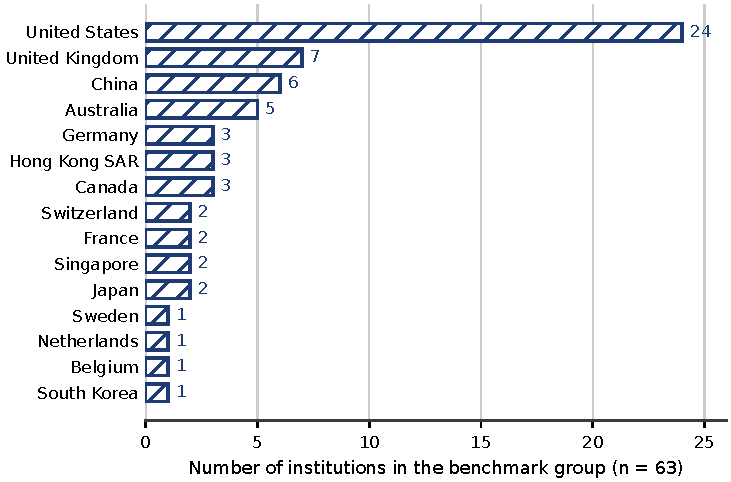
\includegraphics[width=\textwidth]{fig_paises.pdf}
	\caption{Composici\'on del grupo de referencia por pa\'is. El grupo es la cola superior extrema de tres rankings internacionales y no una muestra de las universidades del mundo; v\'ease la Secci\'on~\ref{sec:methods-design}.}\label{fig:paises}
\end{figure}

\begin{figure}[htbp]
	\centering
	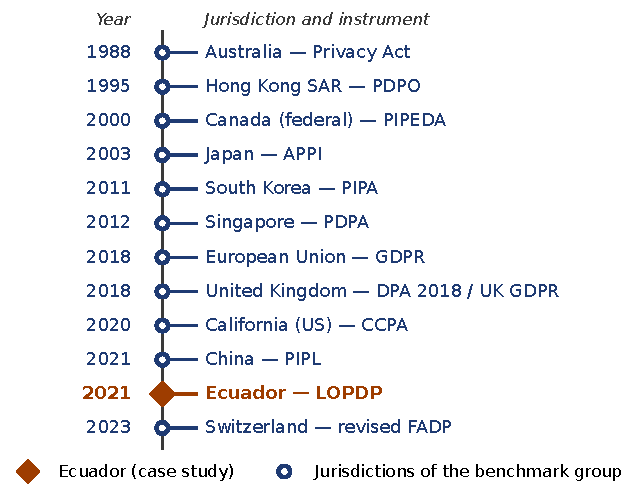
\includegraphics[width=\textwidth]{fig_cronologia.pdf}
	\caption{A\~no en que entr\'o en vigor el r\'egimen general de protecci\'on de datos vigente en cada jurisdicci\'on del estudio. Para los Estados Unidos, que carecen de una ley federal integral, se usa la CCPA de California. El Ecuador pertenece a la oleada m\'as reciente, junto con China.}\label{fig:cronologia}
\end{figure}

\end{appendices}

\bibliography{privacidad_mundo}

\end{document}
